\chapter{Scaling Active Inference}

\section{Introduction}

In this chapter, we consider the application of the free energy principle to action selection, or control, problems. While in the previous chapter on perception, we focused on the process theory of predictive coding, here we focus on the process theory of active inference, and are especially inspired by the discrete state-space active inference theory introduced in Chapter 2. Here, we aim to solve a key limitation of those methods -- their scalability. We propose to do so by parametrizing the key densities of the generative model and recognition distribution by deep neural networks, and then utilizing the tools of deep reinforcement learning to allow active inference agents to scale to levels comparably achieved by contemporary machine learning.

This chapter comprises multiple sections. At the beginning, we give a detailed introduction to reinforcement learning \citep{sutton2018reinforcement}, and especially deep reinforcement learning, as well as the control of inference framework \citep{rawlik2013probabilistic,levine2018reinforcement} from reinforcement learning which also frames the control problem as one of inference. Then we present two studies where we demonstrate that active inference approaches can scale up to be comparable with contemporary deep reinforcement methods. We achieve this scaling by first parametrizing the key distributions in the active inference model by deep neural networks trained through gradient descent, and secondly by approximating the (exponential time) computation of the path integral of the expected free energy either with an amortized neural network prediction, or else through monte-carlo trajectory sampling using a continuous action planning algorithm. In doing so, we create algorithms that are comparable in scalability and performance to current methods in deep reinforcement learning. Additionally, we demonstrate that oftentimes these algorithms can outperform their reinforcement learning counterparts due to the unique properties and insights active inference brings to the table.

In the second section of this chapter, we focus a little more abstractly in trying to understand the difference between model-free and model-based reinforcement learning approaches in terms of inference, and determine that this difference is primarily due to the difference between what we call \emph{iterative} variational inference -- where the parameters of the variational distribution are directly optimized -- and \emph{amortized} inference -- where instead the parameters of a function which outputs the parameters of the variational distribution are optimized. Given this distinction, we first use it to present a taxonomy of a wide range of current reinforcement learning algorithms using a simple two-dimensional quadrant, and secondly, we derive novel algorithms which emerge by combining both iterative and amortized inference together -- an approach we call \emph{hybrid} inference -- which results in powerful algorithms which combine the benefits of each approach, while ameliorating their respective weaknesses.

\subsection{Reinforcement Learning}

The reinforcement learning, or control, problem is one of the most fundamental problems in artificial intelligence and in engineering adaptive systems \citep{sutton1990integrated,sutton1998introduction,kaelbling1996reinforcement,dayan1997using}, and concerns the computation of optimal action \citep{wolpert1997computational,todorov2008general}. The problem is simple. We assume that there is some kind of agent in some kind of environment, and that the agent can take actions which affect the environment \citep{sutton1998introduction}.  Suppose that the agent has some kind of notion of goals or desires that it wants to achieve -- whether these are encoded as a desire distribution, as an objective function, or as rewards given by the environment. The control problem is to compute the optimal action schedule to fulfill the agent's goals. As might be expected, this question has huge applications and implications for an extremely wide range of fields, from machine learning and artificial intelligence (understanding how to make artificial agents act to achieve their goals) \citep{sutton1998introduction,mnih2013playing,silver2016mastering,schrittwieser2019mastering,schulman2015trust} to cognitive science and economics (understanding how humans implement action strategies to achieve their goals) \citep{todorov2008general,wolpert1997computational,dayan2008decision,daw2006cortical} to biology (how do all sorts of biological systems act adaptively) \citep{dayan2009goal,mehlhorn2015unpacking,krebs1978test,pyke1984optimal} to control theory (how to design and program systems which can adaptively regulate and control their environments) \citep{kirk2004optimal,kwakernaak1972linear,sethi2000optimal,kalman1960contributions,johnson2005pid,kappen2005path}.

While this provides an intuitive specification of the control problem, to make real progress we must make it precise mathematically. First, we assume that the environment has states which we denote $x$ and that the agent can emit actions $a$. Secondly, we assume that there exists some reward function which emits rewards $r$ dependent on environmental states $r = f(x)$. The only thing the agent has control over are its actions $a$ which can affect the environment to give it more rewards. We assume that the agent optimizes over \emph{trajectories} of states and actions going into the future, which we denote as $\tilde{x}$, $\tilde{r}$, and $\tilde{a}$. For the moment, to retain full generality, we remain indifferent to whether the agent considers time continuous or discrete, so that $\tilde{x} = \sum_t x(t) = \int dt x(t)$. Finally, we assume that the environmental dynamics and the rewards granted can both be stochastic and can thus be mathematically formalized in terms of probability distributions $p(\tilde{x} | \tilde{a})$ and $p(\tilde{r} | \tilde{x})$. A key advantage of this probabilistic formalism is that it allows us to represent (and remain agnostic between) intrinsic stochasticity in the environment, and the agent's uncertainty about the environment. If the environment or rewards are in fact deterministic and known, we can simply set the distributions to be dirac deltas to recover a deterministic framework. Under this formalism, the objective of the control problem is to maximize \footnote{Here, following the convention in reinforcement learning and economics, we are optimistic and we talk about reward (or equivalently utility) maximization. Control theory, on the other hand, takes a more depressive interpretation and works in terms of minimizing costs. Mathematically, these two formulations are completely equivalent.},
\begin{align*}
\label{control_objective}
\mathcal{L}_{control} &= \underset{a}{argmax} \, \,  \int d\tilde{x} \, p(\tilde{r} | \tilde{x}, \tilde{a})p(\tilde{x} | \tilde{a})p(\tilde{a}) \\
&= \underset{a}{argmax} \, \, \mathbb{E}_{p(\tilde{x} | \tilde{a})p(\tilde{a})}[ \ln p(\tilde{r} | \tilde{x}, \tilde{a})] \numberthis
\end{align*}

Where we can safely take the log of the reward function since log is a monotonic function and does not impact the optimum of the optimization process, but tends to make things nicer numerically. Essentially, what this states is that the control objective is simply to maximize the probability or amount of reward expected under the trajectory of environment states given the agent's trajectory of actions. From this, we can see that to first get a handle on the control problem, we need to understand firstly the environmental dynamics $p(\tilde{x} | \tilde{a})$ and the reward or utility function $p(\tilde{r} | \tilde{x}, \tilde{a})$. We typically represent these dynamics as stochastic differential (or difference) equations depending on whether time is discrete or continuous, as follows,
\begin{align*}
\frac{dx}{dt} = f(x_{1:t},a_{1:t}, \omega) \numberthis
\end{align*}
for continuous time, where $\omega$ is some kind of noise or,
\begin{align*}
x_{t+1} = f(x_{1:T}, a_{1:T}, \omega) \numberthis
\end{align*}
for discrete time. One simplifying assumptions we often make is that the dynamics are Markovian, meaning that the state at time $t+1$ can be computed solely in terms of the state at time $t$ and the action at time $t$, thus that the dynamics become,
\begin{align*}
x_{t+1} = f(x_t, a_t, \omega) \numberthis
\end{align*}
This approach simplifies the analysis considerably. An additional assumption, which is often made, is that the rewards depend only on the state and actions at the current time $p(\tilde{r} | \tilde{x}, \tilde{a}) = \Pi_t p(r(t) | s(t), a(t))$. Under these assumptions the environment of the control problem can be considered to be a Markov Decision Process (MDP). It is also sometimes the case that we assume we do not know the true state of the environment, but are only given access to partial observations $\tilde{o}$ which may not be Markov, even though the hidden states are Markov. The observations are related to the states through a likelihood mapping $p(\tilde{o} | \tilde{x})$. This type of environment is called a Partially-Observed Markov Decision Process (POMDP) \citep{kaelbling1996reinforcement} and is substantially harder to solve optimally than an MDP due to the need to correctly infer the hidden states $\tilde{x}$ from the observations $\tilde{o}$. Nevertheless, the POMDP model has a great deal of generality since, as the state is hidden, it can be whatever is necessary to preserve Markovian dynamics, thus enabling any non-Markovian environment to be written in terms of a Markovian POMDP.

Early approaches to the control problem tried to use methods in variational calculus to directly find analytical solutions to the control problem. Such approaches yielded success in some simple but important, cases, such as Markov linear Gaussian dynamics and quadratic costs. These conditions correspond to dynamics which can be specified as (assuming discrete time),
\begin{align*}
x_{t+1} &= A x_t + B a_t + \omega \\
r_t &= x_t^T Q x_t + a_t^T R a_t \numberthis
\end{align*}
 
Where A, B, Q, and R, are known matrices and $\omega \sim \mathcal{N}(0,\mathbb{I})$ is white Gaussian Wiener noise \citep{wiener2019cybernetics}. In this case, an analytical solution exists in both continuous and discrete time which gives rise to the linear quadratic regulator \citep{kirk2004optimal,kalman1960contributions,kalman1960new}, a centerpiece of modern control theory which is remarkably effective for controlling even complex systems, and for which control solutions can be computed very relatively cheaply and in real time. While the linear dynamics and quadratic costs conditions are quite restrictive (especially the linear dynamics), the linear quadratic regulator approach can be extended somewhat to nonlinear dynamics by simply using a local linearity approximation at every timestep and applying model-predictive control. This iterative LQR \citep{li2004iterative} algorithm, is quite robust and can achieve significant feats of nonlinear control, including use in controlling industrial robotics \citep{feng2014optimization}. Other variational approaches have also been applied and can be quite effective in many cases. For instance, Pontryagin's maximimum principle \citep{kopp1962pontryagin,kirk2004optimal} or `bang-bang' control can be applied productively to find optimal policies in many settings. Recently, there has been advances using path integral methods and the Feynman-Kac lemma to find control solutions for certain classes of nonlinear dynamics \citep{kappen2005path,kappen2012optimal,williams2017information}.

Another approach to the control problem, which can work for arbitrary dynamics, is to simply optimize the control function by gradient descent with respect to the actions. Such an approach goes by the name of policy gradients, since given a policy function $a = f_\phi(s)$ parametrised by parameters $\phi$, we can simply compute gradients of the control problem loss $\frac{\partial \mathcal{L}_{control}}{\partial \phi}$ and optimize the parameters by stochastic gradient descent. The chief difficulty is to propagate gradients through the potentially nondifferentiable and unknown expectation under the environmental dynamics $\mathbb{E}_{p(\tilde{x} | \tilde{a})}$. Luckily, this is achievable through the policy gradient theorem \citep{williams1989learning, sutton1998introduction}
\begin{align*}
    \frac{\partial \mathcal{L}_{control}}{\partial \phi} &= \frac{\partial}{\partial \phi} \int d\tilde{x} \, p(\tilde{x}, \tilde{a}) \ln p(\tilde{r} | \tilde{x}, \tilde{a}) \\
    &=  \int d\tilde{x} \, \frac{\partial}{\partial \phi} p(\tilde{x}, \tilde{a}) \ln p(\tilde{r} | \tilde{x}, \tilde{a}) \\
    &= \int d\tilde{x} \, p(\tilde{x}, \tilde{a}) \frac{\partial \ln p(\tilde{x}, \tilde{a})}{\partial \phi}  \ln p(\tilde{r} | \tilde{x}, \tilde{a}) \\
    &= \mathbb{E}_{p(\tilde{x}, \tilde{a})}[ \ln p(\tilde{r} | \tilde{x}, \tilde{a}) \frac{\partial \ln p(\tilde{x}, \tilde{a})}{\partial \phi}] \numberthis
\end{align*}

Which allows an estimate of the gradient to be computed simply through averages of environmental dynamics. Importantly, this approach does not require knowledge of the true environmental dynamics at all (unlike classical control theory), since we only require samples from the environment which can be obtained simply through interacting with it. Intuitively, we can think of this theorem as saying that the gradient of the control objective is simply the average gradient of the policy, weighted by the rewards received. 

While this method works, the downside is that since the expectation is effectively computed through Monte-Carlo sampling (and generally relatively few samples at that), the gradient estimates generally have a very high variance, which makes learning troublesome and slow. A number of baseline approaches have been invented to try to deal with this problem \citep{sutton2018reinforcement} and to make it more tractable. Nevertheless, policy gradient approaches can be scaled up and applied successfully in challenging tasks, especially continuous control tasks, by parametrizing the policy $f_\phi(x)$ with a deep neural network and directly applying the policy gradient theorem with some additional tricks \citep{schulman2015trust,schulman2017proximal}.

Another approach to the control problem in Markov conditions (but arbitrary dynamics as long as they are Markov) is to use a recursive solution method pioneered by Richard Bellman \citep{bellman1952theory}. He noticed that optimal solutions to the control problem satisfy an interesting recursive relationship -- that the optimal path to the goal at a timestep $t$, must include the optimal path to the goal at a later timestep $t+1$. This property allows you to build up a backwards recursion where you start at the goal at the end and then work backwards, constructing the optimal path in a piecewise fashion from the previous optimal path. The key mathematical quantity, here, is the cost-to-go, which intuitively is the cost of the optimal trajectory from the current position to the goal. In modern reinforcement learning parlance, this cost-to-go is called the optimal value function of a state, and is conversely the expected reward which would be attained from a given state assuming the optimal policy is followed. Written out mathematically, this approach gives rise to the recursive Bellman equation,
 \begin{align*}
\mathcal{V}^*(x_t) = r(x_t) + \mathbb{E}_{p(x_{t+1} | a_t})[\mathcal{V}^*(x_{t+1})] \numberthis
 \end{align*}
which simply states that the optimal value function of a current state, is the reward of the current state plus the maximum average value function of the next state. In effect, if iterated backwards from the end (where the optimal value function is simply $r(x_T)$ and assumed known) this recursion allows you to build up the optimal path by working backwards. If all environmental states and actions are known and finite, then this algorithm can be run explicitly to compute the optimal solution in polynomial time (as opposed to the exponential time approach of just trying all possible paths and picking the best). This is thus a dynamic programming algorithm which is equivalent to other standard dynamic programming algorithms in computer science such as Dijkstra's algorithm for the shortest paths.

Importantly, the Bellman recursion holds not just for the optimal policy and value function, but indeed for \emph{any} policy and value function, this allows solution methods using this recursion to apply even when the state and action space is too large to represent explicitly. In this case, we can write the Bellman recursion as,

 \begin{align*}
 \label{value_update}
\mathcal{V}(x_t) = r(x_t) + \mathbb{E}_{p(x_{t+1} | a_t,x_ts})[\mathcal{V}(x_{t+1})] \numberthis
 \end{align*}

and, without working backwards from the end, we can simply estimate the value functions $\mathcal{V}_\pi(x)$ of a given policy $\pi$ by moving around in our environment, computing rewards and storing the state and the next state, and applying Equation \ref{value_update}. If we do this sufficiently for a given policy, we can then form an estimate of the global value function $\mathcal{V}_\pi(x)$ for all x. With this value function, we can then improve the policy, by simply defining a new policy that takes $\pi = max(r(x_t,a_t) + \mathbb{E}_{p(x_{t+1} |x_t, a_t)}[\mathcal{V}(x_{t+1})]$. Somewhat surprisingly, it has been proven that if the estimated value function is accurate, then the new policy defined in such a manner is necessarily the same or better (in terms of average reward obtained from the MDP) than the previous policy, and that if we iterate the process of sampling new states to estimate the value function, and then improving the policy, then we will converge upon the optimal policy $\pi^*$ \citep{sutton2018reinforcement}. This approach, called policy iteration, is the cornerstone of classic reinforcement learning algorithms such as temporal difference learning \citep{sutton1988learning}, and SARSA \citep{sutton1996generalization,singh1996reinforcement}.

 A closely related approach is called Q-learning \citep{watkins1992q}, which instead of using the value function, instead maintains an estimate of the state-action value function $Q(x,a)$, which is called the Q-function for historical reasons. The Q function satisfies a similar recursive relationship to the value function,
\begin{align*}
\mathcal{Q}(x_t,a_t) = r(x_t,a_t) + \underset{a_t}{argmax} \mathbb{E}_{p(x_{t+1},a_{t+1} | a_t,x_t})[\mathcal{Q}(x_{t+1},a_{t+1})]
\end{align*}

 Given an estimate of the Q function, the policy improvement step is simple. $\pi^{t+1} = \underset{a}{arg max} \, Q(s,a)$. The Q-learning algorithm combines both policy evaluation (estimating the value or Q function) and policy improvement into one continuous algorithm, which can be simply defined as,
 \begin{align*}
 a(x_t) &= max_{a_t} Q(x_t,a_t) \\
Q(x_t,a_t) &= r(x_t,a_t) + max_{a_{t+1}} \mathbb{E}_{p(x_{t+1} | x_t,a_t)}[\mathcal{Q}(x_{t+1},a_{t+1})] \numberthis
 \end{align*}
The Q-learning algorithm is extremely popular and effective and has been central to many major successes of reinforcement learning, from playing backgammon \citep{tesauro1994td} to Atari \citep{mnih2013playing,schrittwieser2019mastering}. The Q function and value function can be related straightforwardly by $\mathcal{V}(x) = \int da \mathcal{Q}(x,a)$ -- i.e. the value function is simply the Q function averaged over all actions. Another approach is to write everything instead in terms of an \emph{advantage function} $\mathcal{A}(x,a) = \mathcal{Q}(x,a) - \mathcal{V}(x)$ which simply subtracts the action-independent value function baseline from the Q-value, effectively normalizing it, since the only important thing from the perspective of Q learning is the \emph{relative values} of each action. This approach reduces the gradient variance when trying to estimate the Q function and often makes the resulting algorithms more stable \citep{hessel2018rainbow}.

 In classical reinforcement learning we typically represent the Q and value function explicitly in discrete-state and discrete-action environments. For instance, with discrete states, the value function $\mathcal{V}(x)$ would simply be a vector of length $\mathbb{S}$ where $\mathbb{S}$ is the number of distinct states. The Q function $\mathcal{Q}(x,a)$ is simply an $\mathbb{S} \times \mathbb{A}$ matrix where $\mathbb{A}$ is the action dimension. 

 Another useful representation is the successor representation \citep{dayan1997using}. This approach rewrites the value function in terms of the instantaneous reward $r(x)$ and a successor matrix $\mathcal{M}(x, x')$ which is a $\mathbb{S} \times \mathbb{S}$ matrix which represents the average transition probabilities for a given policy from state $x$ to state $x'$. This matrix $\mathcal{M}$ can be thought of as the stationary transition distribution of the Markov chain for a given policy. The value function can be decomposed into,
 \begin{align*}
\mathcal{V}(x) = \mathcal{M}(x,x')r(x) \numberthis
 \end{align*}

 The successor representation, crucially, by separating out the policy-dependent component (M) from the reward $r$ allows for computation of different value functions for a given policy rapidly under different reward functions. Thus this representation allows for very flexible changes of behaviour given a change in reward. Of course the optimal policy also changes under a change of reward function, and this change cannot be straightforwardly determined solely by the successor representation.

\subsection{Deep Reinforcement Learning}                                                                                  

While classical reinforcement learning approaches typically represent the value or Q functions explicitly as vectors and matrices, such methods only work for relatively small and discrete state and action spaces, and cannot easily scale to the extremely large state and action spaces required for playing complex games as well as for complex continuously valued action spaces such as in robotics, where simply discretizing the space with a sufficiently fine grid will simply result in too many states to handle. Therefore, to maintain scalability, instead of explicitly representing the state and value functions, it becomes necessary to approximate them with powerful function approximators. While other approaches using linear features \citep{baird1995residual,gordon1995stable}, or nonlinear basis function kernels \citep{doya2000reinforcement} are possible, recent systems have overwhelmingly used deep neural networks to approximate the value or Q functions directly. To make this explicit, instead of representing the value function $\mathcal{V}[x]$ as a vector, we instead represent it as a function $\mathcal{V}_\psi(x)$ which takes a state $x$ and maps it to a scalar value. This function is implemented by a deep neural network with parameters $\psi$. We can then learn these parameters using stochastic gradient descent on a loss function which is a modified version of the Bellman recursion,
\begin{align*}
\label{valuenet_equation}
\mathcal{L}_{Valuenet}(x) = (\mathcal{V}_\psi(x) - r(x) - max_a \mathbb{E}_{p(x' | x,a)}[\mathcal{V}_\psi(x')]))^2 \numberthis
\end{align*}
which is the squared residual between the value predicted for a state $x$ by the value network, and the value predicted by the Bellman recurrence relation. By using this approach, therefore, we utilize the intrinsic generalization capabilities of deep neural networks to allow us to estimate value or Q functions for an otherwise intractably large space. This approach can be straightforwardly extended to Q-learning and other Bellman based methods. Similarly, applying policy gradients with deep neural networks is even simpler -- we simply parametrise the policy $q_\psi(a | s)$ with a deep neural network with parameters $\psi$ and train it directly using stochastic gradient descent on the policy gradient objective \citep{schulman2015trust,schulman2017proximal}. 

To get this approach working well in practice, however, requires quite a number of tricks. For instance, the neural networks cannot be trained simply through continuous interaction with the environment, as this gives rise to correlated data which leads to overfitting and catastrophic forgetting within the value network \citep{mnih2013playing}. Thus, instead, it is necessary to make the data fed into the network as $i.i.d$ as possible by using a memory replay buffer, which stores all experience the agent has encountered over its lifetime and then replays it at random to be optimized according to Equation \ref{value_update} \citep{mnih2013playing}.  Similarly, note that in the value network update equation (Equation \ref{valuenet_equation}), the parameters of the value network appears twice -- once computing the value of $x$ and again computing the values of $x'$. It has been found empirically, that this leads to instabilities in the optimization process which often destroy learning, since the optimization process is effectively chasing a set of moving targets. To resolve this problem, the value estimates of $x'$ are often computed using a `frozen' value network which is not optimized directly, but is a copy of the value network from some number of iterations past. The frozen network is then updated to match the current value network every given number of iterations \citep{mnih2015human}. Another issue is that the value estimates are often skewed extremely positive due to the max operator in the objective interacting inaccurate value function estimates. This can be ameliorated empirically by simply training two (or many) value networks in parallel, and then choosing the smallest value estimates out of all of them, a technique known as dueling value networks \citep{wang2016dueling}. For a thorough review of tricks and tips for training deep reinforcement learning agents, we suggest \citet{fujimoto2018addressing,hessel2018rainbow}.

Nevertheless, once all of these instabilities have been addressed, the result is an extremely powerful and general learning technique which has been demonstrated empirically to scale up to solve very challenging tasks such as Atari games \citep{mnih2015human,mnih2014neural} and Go \citep{silver2016mastering,silver2017mastering}, Starcraft II \citep{vinyals2019grandmaster}, and ultimately very challenging tasks in robotics \citep{nagabandi_neural_2017,nagabandi2019deep,chua_deep_2018,williams2017model}. 

\subsection{Model-free vs Model-based}

It is important to note that all the methods we have discussed so far require samples from the true environmental dynamics to approximate the expectation $\mathbb{E}_{p(\tilde{x}, \tilde{a})}$ from the ultimate loss function (Equation \ref{control_objective}. While these samples are easy to acquire in the case where interacting with the environment is cheap and easy, such as when the environment is a simulation such as a game or an OpenAI gym environment \citep{brockman2016openai}, in many real world tasks this is not the case. For instance, in robotics, interacting with the real environment is often slow (the real robot has to actually move or do things in physical space) and costly (this movement requires power and also induces wear and tear on the robot. In extreme situations, bad policies may actually result in the robot damaging itself). In this case, it is often better if we can somehow eschew interacting with the real environment in favour of a model of the real environment. Having a `world model' \citep{ha_recurrent_2018} of the environment allows the agent to plan and test different potential courses of action without having to sustain costly and slow interactions with the real world. The utility of models does not just extend to the environmental dynamics. It is often the case that the actual \emph{reward function} of the agent is unknown. This is not generally true in reinforcement learning and control theory, which typically have well specified rewards, but is often true in the case of biological organisms encountering novel contingencies, where it is not necessarily known a-priori if a situation is good or bad. Thus, we can also learn a model of the reward function as well.

Mathematically, we can formalize this property of having a model of the transition dynamics or reward functions by postulating additional probability densities which the agent possesses $q_\phi(\tilde{x} | \tilde{a})$ and $q_\theta(\tilde{r} | \tilde{x}, \tilde{a})$ which represent the agent's model of the true environmental dynamics $p(\tilde{x} | \tilde{a})$ and true reward function $p(\tilde{r} | \tilde{x}, \tilde{a})$. Then, using importance sampling, we can introduce these models into the previous loss function,
\begin{align*}
\mathcal{L}_{control} &= \underset{a}{argmax} \, \mathbb{E}_{p(\tilde{x} | \tilde{a})p(\tilde{a})}[ \ln p(\tilde{r} | \tilde{x}, \tilde{a})] \\
&= \underset{a,\phi,\theta}{argmax} \, \mathbb{E}_{p(\tilde{x} | \tilde{a})p(\tilde{a})} \frac{q(\tilde{x} | \tilde{a})}{q(\tilde{x} | \tilde{a})}    [ \ln p(\tilde{r} | \tilde{x}, \tilde{a}) \frac{q(\tilde{r} | \tilde{x}, \tilde{a})}{q(\tilde{r} | \tilde{x}, \tilde{a})}] \\
&= \underset{a,\phi,\theta}{argmax} \, \mathbb{E}_{q(\tilde{x} | \tilde{a})p(\tilde{a})} \frac{p(\tilde{x} | \tilde{a})}{q(\tilde{x} | \tilde{a})}    [ \ln q(\tilde{r} | \tilde{x}, \tilde{a}) \frac{p(\tilde{r} | \tilde{x}, \tilde{a})}{q(\tilde{r} | \tilde{x}, \tilde{a})}] \\
&= \underset{a,\phi, \theta}{argmax} \, \mathbb{E}_{q(\tilde{x} | \tilde{a})p(\tilde{a})} \ln \frac{p(\tilde{x} | \tilde{a})}{q(\tilde{x} | \tilde{a})}    [ \ln q(\tilde{r} | \tilde{x}, \tilde{a}) \frac{p(\tilde{r} | \tilde{x}, \tilde{a})}{q(\tilde{r} | \tilde{x}, \tilde{a})}] \\
&= \underset{a,\phi, \theta}{argmax} \, \underbrace{\mathbb{E}_{q(\tilde{x} | \tilde{a})p(\tilde{a})} [ \ln q(\tilde{r} | \tilde{x}, \tilde{a}) ]}_{\text{Reward Maximization}}  - \underbrace{KL[q(\tilde{x} | \tilde{a}) || p(\tilde{x} | \tilde{a})]}_{\text{System Identification}}  -  \underbrace{\mathbb{E}_{q(\tilde{x} | \tilde{a})p(\tilde{a})} \big[ \frac{q(\tilde{r} | \tilde{x}, \tilde{a})}{p(\tilde{r} | \tilde{x}, \tilde{a})}}\big]_{\text{Reward Model Identification}} \numberthis \\
\end{align*}

Here we see that the objective can be partitioned into three terms. The first, reward maximization, is equivalent to the original control objective except it utilizes the model environmental dynamics and reward function instead of the true environmental dynamics and reward function. The second term, `system identification', encodes the KL divergence between the true and modelled environmental dynamics, and is minimized with respect to the parameters of the model of the dynamics. Optimizing this term encourages the agent to learn an accurate dynamics model of the world. The third term, `reward model identification' encourages the reward model to match the true reward function and optimizing this term with respect to the parameters of the reward model minimizes the difference between the model reward distribution and the true reward distribution.

Interestingly, mathematically, the minimization of all of the three parameters is over all three terms. This leads to, for instance, the parameters of the reward and dynamics model to be optimized over the reward maximization term, which effectively encourages the dynamics and reward models to try to learn positively biased dynamics and reward models which are encouraged to give out larger rewards. Conversely, the divergence terms between true and modelled environmental dynamics and reward function are also being optimized with respect to action, so the optimisation process also encourages action to make the true dynamics and true reward function correspond more closely to the modelled ones. These interactions between the optimizations of the different terms often have strange and deleterious effects on agent behaviour, especially learning the dynamics to maximize the reward, which can give agents a highly dysfunctional `optimism bias' \citep{levine2018reinforcement}. As such, in practice, this optimization is often split into three separate and independent optimizations for each set of parameters respectively,
\begin{align*}
& \underset{a}{argmax} \, \, \mathbb{E}_{q(\tilde{x} | \tilde{a})p(\tilde{a})} [ \ln q(\tilde{r} | \tilde{x}, \tilde{a})  \numberthis \\
& \underset{\phi}{argmin} \, \,  KL[q_\phi(\tilde{x} | \tilde{a}) || p(\tilde{x} | \tilde{a})]  \\
& \underset{\theta}{argmin} \, \, \mathbb{E}_{q(\tilde{x} | \tilde{a})p(\tilde{a})} \frac{q(\tilde{r} | \tilde{x}, \tilde{a};\theta)}{p(\tilde{r} | \tilde{x}, \tilde{a})} \numberthis
\end{align*}

These three optimization processes correspond to maximizing the reward (standard reinforcement learning), learning the environmental dynamics model, and learning the reward function, respectively. In control theory, the process of learning a dynamics model is called system identification. 

Given good reward and dynamics models, it is then possible to utilize standard model-free reinforcement learning approaches to estimate Q and value functions, or estimate policy gradients directly through simulated samples of the dynamics model. With these it is then possible to learn policies in the usual way without ever having to interact with the environment (except to learn the models in the first place). This approach, first introduced in the Dyna architecture \citep{sutton1991dyna} has been studied in the literature for a long time, and is generally more sample efficient than pure model-free reinforcement learning which learns directly from environmental transitions, as learning dynamics models of the world is typically faster than learning reward models, since the prediction errors in the state of the world is a richer informational signal than the reward prediction error since the reward is usually scalar while the world-state is typically very high dimensional.

Another approach, once you have a model is to skip the model-free methods and move directly to planning using the model. In the simplest case, this can be done by sampling different action trajectories, simulating their consequences and rewards using the dynamics and reward models, and then simply choosing the action trajectory with the best estimated rewards. More advanced methods include the cross-entropy method, which tries to fit a probabilistic (Gaussian) action distribution to maximize rewards, and the path-integral method, which fits a Boltzmann distribution of action trajectories over rewards \citep{kappen2012optimal,rawlik2013probabilistic,theodorou2010reinforcement,williams2017model,williams2018predictive}. This kind of model-based planning is often combined with Model-Predictive-Control, which is simply where you re-plan fully at every time-step, and has been used to reach state of the art performance on a wide variety of reinforcement learning \citep{nagabandi2019deep} and robotics tasks \citep{williams2016aggressive,williams2017information}, all while requiring substantially fewer environmental interactions than model-free reinforcement learning approaches.

\subsection{Exploration and Exploitation}

An interesting question that arises in the control problem, wherever there are any unknowns, either of the optimal value function and policy or the environmental dynamics and reward function, is the exploration-exploitation tradeoff \citep{cohen2007should,dayan2008decision,sutton1998introduction,kaelbling1998planning,mobbs2018foraging,berger2014exploration}. This trade-off arises because in order to obtain a more accurate estimate, it is usually necessary to explore new regions of the state-space away from the locally optimal location. However, by ignoring the locally optimum course of action, you incur an opportunity cost equal to the difference between the (usually worse) reward from the exploring compared to the local optimum. Conversely, by only ever exploiting the local optimum and never exploring, if there are actually better optima out there, which you have simply not found, you incur a constant opportunity cost of the distance to the true optimum every single time you exploit your local optimum. Thus, to find the truly optimal behaviours, it is necessary to explore widely, and not just be sucked into whatever the closest local optima you find. However, exploration has an intrinsic cost associated with it, since assuming you have a halfway decent local optimum, almost everything you explore will be worse than that, and thus exploration must be kept to a minimum to maximize return, even in the long run.

The exploration-exploitation tradeoff is also central to the behaviour and performance of reinforcement learning agents, especially deep reinforcement learning agents which cannot explicitly represent every contingency in the state-space. Empirically, it has been found that except in extremely simple tasks, or where the reward function is a smooth gradient to the global optimum, some forms of exploration are necessary to achieve good performance with deep reinforcement learning techniques. A large number of heuristic exploration techniques have been developed in the literature which work well for many tasks. Perhaps the simplest of these is the $\epsilon$-greedy approach \citep{sutton1998introduction}, which simply takes the greedy action $(1 - \epsilon)$ amount of the time, and takes a random action $\epsilon$ percent of the time, where $\epsilon$ is a small number -- typically about $0.02-0.05$. This method essentially bakes in a certain degree of random exploration into the method so that it will (eventually) explore all contingencies purely due to its random actions. In many control tasks this method generates sufficient exploration to enable good performance. More sophisticated variants anneal the value of $\epsilon$ over time; working on the idea that at the beginning when little is known you should explore more, and then later when you already have a pretty good policy you should explore less. Another approach in algorithms like Q learning is that instead of simply taking the maximum value, take actions with a probability equal to their softmaxed Q-values -- $q(a | x) = \frac{\beta exp(-\mathcal{Q}(a | x))}{\sum_a exp(-\mathcal{Q}(a | x))}$ where $\beta$ is a parameter which controls the spread or entropy of this distribution. When $\beta$ is large, then the distribution is highly peaked and tends towards the max. When $\beta$ is small, then the distribution tends towards a uniform over all action possibilities. This method is called Boltzmann exploration \citep{cesa2017boltzmann}, since the action distribution is equivalent to the Boltzmann distribution of statistical mechanics with the $\beta$ parameter functioning as an inverse temperature.

Another approach, which we will explore in detail in the next section, is to add an entropy maximization term to the objective \citep{levine2018reinforcement}. Thus, instead of simply maximizing the reward, the goal is to maximize the reward while keeping the entropy of the policy as great as possible, and thus making action as random as possible \footnote{This idea is similar to, but distinct from, ideas such as upper-confidence-bound sampling which assign optimism bonuses to states in proportion to the inverse degree to which they have been sampled. The key difference is that maximum entropy approaches provide bonuses to actions based on the overall entropy of the action distribution while UCB algorithms provide bonuses to states based on their epistemic uncertainty.} While still a random kind of exploration, this performs better than $\epsilon$ greedy approaches since it explicitly trades off randomness and reward maximization in the objective, rather than as an $\epsilon$ parameter that needs to be tuned by hand.

While all these exploration methods work well in practice in many benchmark environments for deep reinforcement learning, they all fundamentally utilize \emph{random exploration} -- i.e. actions are selected randomly in order to drive exploration. It is important to note, however, that this strategy is necessarily very inefficient, since even with purely random actions, a random walk will explore slowly. Indeed, these methods tend to perform rather poorly in more challenging large environments where all useful contingencies cannot realistically be explored with a random walk in a reasonable amount of time, and tend to perform especially poorly in \emph{sparse reward} environments, where rewards are hard to obtain and often require a pretty good policy to even get any reward at all \citep{tschantz2020reinforcement}. A good example of such an environment is many games, where you are only rewarded a 1 if you win the game. However, to even win any games at all requires some skill at playing \footnote{This is often addressed in practice by using reward shaping, where typically either the agent designer or the environment designer will create a `proxy' reward function for the real one which is less sparse. For instance, in a game like chess, instead of simply rewarding winning or losing the game, the agent might get rewards for taking pieces, or gaining positional advantage. While this approach works very well in practice, it requires human intervention for every task the agent tries to accomplish, and is often tricky to design a proxy reward which successfully leads to the correct ultimate behaviour. Ultimately, we want agents to be able to interact with the world fully autonomously, which means that they should not need special human-designed reward functions to handle any new situation, and so we do not consider reward shaping further}. To address the shortcomings of random exploration, a significant amount of work has been done on \emph{directed}, or information-seeking, exploration. Here, exploratory actions are not completely random but instead directed at some exploratory goal -- usually to accumulate information or to resolve uncertainty about the world. This makes sense as in a stationary environment there is little point in repeatedly exploring bad options which are known to be bad. The key is to explore where there is remaining resolvable uncertainty. 

A number of different objectives, or `intrinsic measures' \citep{oudeyer2009intrinsic} have been proposed to achieve this. These include prediction error minimization \citep{pathak2017curiosity}, ensemble divergence \citep{chua_deep_2018}, explicit information gain \citep{shyam_model-based_2019,tschantz2020reinforcement,sun_planning_2011}, and empowerment \citep{klyubin2005empowerment}. Typically such approaches postulate a separate `exploration objective' and then either operate in two phases whereby first the model optimizes the exploration objective, and then it switches to optimizing the greedy objective \citep{shyam_model-based_2019}, or alternatively, the exploration and greedy objectives are added together to form a unified objective function which is minimized throughout \citep{tschantz2020reinforcement}. Such approaches therefore encourage the agent to seek a balance between its exploratory and reward-maximization imperatives. This has the theoretical advantage of encouraging the agent to only explore regions of the state-space which combine both a high expected reward \emph{and} much resolvable uncertainty, as opposed to simply resolving uncertainty for its own sake. In the literature, most of these exploratory objectives are simply postulated and argued for on intuitive grounds and then empirically compared. However, with the exception of the entropy maximization discussed above, which we shall see arises from explicitly considering control as a variational inference problem, the mathematically principled origins of these additional exploratory terms, especially information-gain and empowerment terms remains mysterious. Chapter 5 is dedicated to deriving the mathematical basis for such objectives.

\subsection{Control as Inference}

Since we have been so interested in understanding brain function through the lens of Bayesian (variational) inference in this thesis, a natural question arises as to whether the control problem as discussed previously can be cast in such an inference framework. It turns out that this is indeed the case, and is quite straightforward to achieve. Starting from \citep{attias2003planning} and then developed by \citep{toussaint2006probabilistic,todorov2008general,rawlik2013probabilistic,kappen2012optimal,theodorou2010generalized,levine2018reinforcement}, a small line of the literature has worked on investigating and developing the close connections between the control problem and Bayesian inference.
\begin{figure}
    \begin{center}
          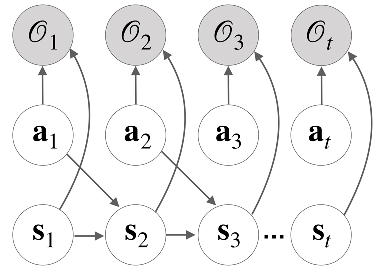
\includegraphics[width=0.35\textwidth]{chapter_4_figures/pgm.pdf}
    \end{center}
    \caption{Graphical model for control as inference, with optimality variables $\Omega$. Other than the optimality variables, the graphical model takes the form of a Markov Decision Process with actions $a$ and states $s$. The state of a specific timestep depends on the action and state of the last time-step. By writing out an explicit graphical model like this, we can apply a whole field's worth of inference algorithms on graphical models like this to solve control problems.}
\label{fig:graphical-model}
\end{figure}

While the control objective (Equation \ref{control_objective} is a probabilistic objective, it is not yet an \emph{inference} objective. There is nothing there to be inferred. The key step is to define dummy variables $\Omega_{1:T}$ which are binary random variables which simply whether a given trajectory timestep is optimal or not. $\Omega_t = 1$ if the timestep is optimal and $\Omega_t = 0$ if it is not optimal. Given this dummy variable, the task of inferring the optimal policy can be written simply as finding the distribution $p(\tilde{a}, \tilde{x} | \tilde{\Omega} = 1)$. To begin inferring this distribution, it is first necessary to make one more assumption about the dummy variables $\Omega$, in order to operationalize the notion of optimality. We define $p(\Omega_t = 1 | a_t, x_t) \propto exp(-r(x_t, a_t))$ such that the probability of optimality is proportional to the exponentiated reward. Intuitively, this can be seen as a mathematical trick allowing the `log-likelihood of optimality' to be equal to the reward, thus allowing us to cast reward maximization as a process of maximum likelihood estimation.

One way we can find the crucial distribution is simply to directly compute it via Bayes rule. First, we write out Bayes rule explicitly,
\begin{align*}
p(a_t | x_t, \tilde{\Omega}) &= \frac{p(\tilde{\Omega}, x_t, a_t)}{p(\tilde{\Omega}, x_t)} \\
&= \frac{p(\tilde{\Omega}| x_t, a_t)p(a_t | x_t)p(x_t)}{p(\tilde{\Omega} | x_t)p(x_t)} \\
&= \frac{p(\tilde{\Omega}| x_t, a_t)p(a_t | x_t)}{p(\tilde{\Omega} | x_t)} \\
&\approx \frac{p(\tilde{\Omega}| x_t, a_t)}{p(\tilde{\Omega} | x_t)} \numberthis
\end{align*} 
Where, in the final line, we assume that the action prior $p(a_t | x_t)$ is uniform. Now, looking at the two terms we have left, we can intuitively think of the numerator $p(\tilde{\Omega}| x_t, a_t)$ as representing the probability of optimality of all future states, given the current state and action. However, we have another term for this -- the cost-to-go, or the Q-function. In effect, we obtain the Bellman recursive relationship directly from Bayes rule. Secondly, the denominator $p(\tilde{\Omega} | x_t) = \int d a_t \, \, p(\tilde{\Omega}| x_t, a_t)$ clearly corresponds to the value function.

We can from this directly derive recursive relationships among these terms,
\begin{align*}
    p(\Omega_{t:T}| x_t, a_t) = \int dx_{t+1} da_{t+1} \, p(\Omega_{t+1:T} | x_{t+1}, a_{t+1}) p(x_{t+1}, a_{t+1} | x_t, a_t) p(\Omega_t | x_t, a_t) \numberthis
\end{align*}
We can thus see, that due to our definition of optimality that $p(\Omega_t | x_t, a_t) = exp(-r(a_t, x_t)$, that to obtain the correspondence to the value and Q function requires the \emph{log} of the optimality probability. We thus have,
\begin{align*}
    & \mathcal{Q}_{CAI} = \ln p(\Omega_{t:T}| x_t, a_t) \\
    & \mathcal{V}_{CAI} = \ln p(\Omega_{t:T}| x_t) \numberthis
\end{align*}
Where, by taking the log of the integral and exponential, we effectively have the log-softmax function instead of the max in the Bellman equations. This corresponds to a `soft' maximum instead of the hard maximum used in the traditional Bellman recursion. However, other than that, our new definitions of the value and Q function satisfy the standard Bellman recursive relationship, and as such can be used to derive all the traditional reinforcement learning algorithms such as Q-learning, temporal difference learning, and SARSA \citep{sutton1996generalization}.

Another approach is to use variational inference and attempt to approximate the true posterior distribution given optimality $p(\tilde{a}, \tilde{x} | \tilde{\Omega})$ with a variational distribution $q(\tilde{x}, \tilde{a})$. To make this approximation accurate, we thus wish to minimize the divergence between the two distribution.
\begin{align*}
\mathcal{L}_{CAI} &= \KL[q(\tilde{x}, \tilde{a}) || p(\tilde{x}, \tilde{a} | \tilde{\Omega})] \\
&= \KL[q(\tilde{x}, \tilde{a}) || \frac{p(\tilde{x}, \tilde{a}, \tilde{\Omega})}{\tilde{\Omega}}] \\
&= \underbrace{\KL[q(\tilde{x}, \tilde{a}) || p(\tilde{x}, \tilde{a}, \tilde{\Omega})]}_{\text{ELBO}}+ \ln \tilde{\Omega} \numberthis
\end{align*}

Where we only need to optimize the Evidence Lower Bound (ELBO) term since $\ln \tilde{\Omega}$ is constant with respect to the variational density $q(\tilde{x}, \tilde{a})$. Crucially, we can then split up the ELBO term as follows,
\begin{align*}
\mathcal{L}_{CAI} &= \KL[q(\tilde{x}, \tilde{a}) || p(\tilde{x}, \tilde{a}, \tilde{\Omega})] \\
&= \KL[q(\tilde{a} | \tilde{x})q(\tilde{x}) || p(\tilde{\Omega} | \tilde{x}, \tilde{a})p(\tilde{a} | \tilde{x})p(\tilde{x})] \\ 
&= \underbrace{\mathbb{E}_{q(\tilde{x},\tilde{a})}[\ln p(\tilde{\Omega} | \tilde{x}, \tilde{a})]}_{\text{Reward Maximization}} + \underbrace{\KL[q(\tilde{a} | \tilde{x}) || p(\tilde{a} | \tilde{x})]}_{\text{Action Divergence}} + \underbrace{\KL[q(\tilde{x}) || p(\tilde{x})]}_{\text{Dynamics Divergence}} \numberthis
\end{align*}

If we then assume that the variational dynamics $q(\tilde{x})$ are equal to the true environmental dynamics $p(\tilde{x})$ (the agent cannot change the dynamics except through action) then the action divergence term disappears. Additionally, if we use the fact, defined earlier, that $p(\tilde{\Omega} | \tilde{x}, \tilde{a}) = \prod_t exp(-r(a_t, x_t))$, then we obtain an objective which looks substantially more similar to traditional reinforcement learning objectives except for an additional action divergence term between the variational action distribution (the policy) and a prior action distribution.
\begin{align*}
\mathcal{L}_{CAI} &= \underbrace{\mathbb{E}_{q(\tilde{a} | \tilde{a})p(\tilde{x})}[\prod_t^{T} r(x_t, a_t)]}_{\text{Reward Maximization}} + \underbrace{\KL[q(\tilde{a} | \tilde{x}) || p(\tilde{a} | \tilde{x})]}_{\text{Action Divergence}} \numberthis
\end{align*}

If we further assume a uniform action prior, then the control as inference objective reduces to,
\begin{align*}
\mathcal{L}_{CAI} &= \mathbb{E}_{q(\tilde{a} | \tilde{a})p(\tilde{x})}[\prod_t^{T} r(x_t, a_t)] - \mathbb{H}[q(\tilde{a} | \tilde{x})] \\
&= \mathbb{E}_{q(\tilde{a} | \tilde{a})p(\tilde{x})}[\prod_t^{T} r(x_t, a_t) - \ln q(a_t | x_t)] \numberthis
\end{align*}

Which is simply reward maximization while also simultaneously maximizing the entropy of the policy $q(\tilde{a} | \tilde{x})$. This objective has been utilized in a number of recent works \citep{rawlik2013stochastic,haarnoja2017reinforcement,haarnoja2018soft,abdolmaleki2018maximum}, and forms the basis of the soft-actor critic architecture \citep{haarnoja2018soft}, which simply optimizes a relatively standard actor-critic architecture on this objective. It has been found to reach state-of-the-art performance for model-free reinforcement learning on a wide range of challenging continuous control tasks \citep{hessel2018rainbow,haarnoja2018applications}. Moreover, the simplicity and robustness of this algorithm allow it to serve as an influential benchmark for the field. This CAI objective can be straightforwardly optimized by taking gradients of $\mathcal{L}_{CAI}$ against whatever parameters there are. For instance, optimizing the control-as-inference objective is identical to standard policy gradients except that each reward the agent receives has $\ln q(a_t | x_t)$ subtracted from it. This differentiates control as inference from previous works \citep{o2017deep}, which heuristically used an entropy regulariser to prevent policy collapse, but computed the entropy directly outside of the expression for the reward. The control-as-inference objective is both simpler to implement and more robust than this method.

Importantly, the control as inference objective, as it is a variational bound, can be derived directly from, and as a lower bound on the marginal likelihood of optimality $\ln p(\tilde{\Omega})$. The derivation is straightforward and goes as follows,

\begin{align*}
\ln p(\tilde{\Omega}) &= \ln \int p(\tilde{\Omega}, \tilde{x}, \tilde{a}) \frac{q(\tilde{a} | \tilde{x})}{q(\tilde{a}, \tilde{x})} \\
&\leq \mathbb{E}_{q(\tilde{a}, \tilde{x})}[\frac{p(\tilde{\Omega}, \tilde{x}, \tilde{a})}{q(\tilde{a}, \tilde{x})}] \\
&\leq \mathbb{E}_{q(\tilde{a} | \tilde{x})p(\tilde{x})}[\frac{p(\tilde{\Omega} | \tilde{x}, \tilde{a})p(\tilde{a} | \tilde{x})}{q(\tilde{a}| \tilde{x})}] \\
&\leq \mathbb{E}_{q(\tilde{a} | \tilde{x})p(\tilde{x})}[\prod_t^T r(x_t, a_t)] - \KL[q(\tilde{x} | \tilde{a}) || p(\tilde{a} | \tilde{x})] \\
&\leq \mathcal{L}_{CAI} \numberthis
\end{align*}

Under the assumption that the variational and generative dynamics are the same. Overall, the control as inference approach demonstrates that it is possible, even relatively straightforward, to derive a range of reinforcement learning algorithms from a variational approach on an MDP graphical model augmented with additional optimality variables. Doing so results in the standard reward maximization objective plus a regularisation term which tries to keep the learned policy $q(\tilde{a} | \tilde{x})$ as close as possible to some action prior $p(\tilde{a} | \tilde{x})$. If the action prior is set to be uniform, then this regularising KL divergence simply reduces to the maximization of the entropy of the action policy. This action entropy maximization term functions as a powerful regulariser and implicit exploratory drive, which aims to keep the policy as random as possible while still maintaining performance. This term is especially powerful and important for preventing policy collapse, a well-known phenomenon in policy gradient and actor-critic methods \citep{fujimoto2018addressing}, in which the probabilistic policy of an agent typically collapses to some deterministic policy which may not even be very good. Once it is in this state, it is very difficult for the agent to continue to explore to find better policies, since it has minimal probability of taking other actions. The theoretical benefits of this action entropy term have been demonstrated empirically in the literature, where `soft' control as inference approaches have generally shown to outperform classical reinforcement approaches as well as being more stable and easy to train. However, it is important to note that although the action entropy term is effective at maintaining exploration, it only encourages \emph{random} exploration, or random walk behaviour in action-space. To solve sparse reward tasks in a reasonable amount of time, it is possible that a more intelligent, \emph{directed} exploration strategy is needed, which focuses explicitly on minimizing resolvable uncertainty about the world. Such information-seeking exploration objectives are a major focus and benefit of active inference, and understanding their mathematical nature and origins is the major task of Chapter 5 of this thesis.

\section{Deep Active Inference}

Active inference and reinforcement learning both purport to solve the same fundamental problem -- that of adaptive action selection to maximize some notion of rewards or desires, given uncertainty about the world and about the optimal policy to take. While active inference arises from the paradigm of variational Bayesian inference with posterior policy distributions and complex generative world models \citep{friston_active_2015,friston2017process}, reinforcement learning arises primarily from the Bellman equation and the recursive properties of optimality \citep{sutton2018reinforcement,kaelbling1996reinforcement}, and utilizes constructs such as value functions and policy networks to learn adaptive behaviour even on challenging and complex control tasks.

Despite the very different origins of the two fields, since they are fundamentally trying to solve the same problem, it seems likely that there is much each field can learn from the other, since they both illuminate difference facets of the same reality. Specifically, the discrete-state-space active inference models introduced previously, in Chapter 2, suffer from many limitations of scale. Specifically, they represent the core distributions as discrete categorical variables, which require a relatively small, discrete and known state-space to function. Moreover, active inference models typically assume knowledge of the true generative process (i.e. the likelihood and prior matrices (A and B)), which often cannot simply be assumed in more realistic control tasks. \footnote{There is some work empirically investigating learning the A matrix using dirichlet hyperpriors over its values \citep{schwartenbeck_computational_2019}, and the rules for learning the B matrix are also straightforward. However, most of the active inference literature eschews these methods in favour of hand-designed likelihood and transition matrices \citep{friston_active_2015,friston2012active,parr2017uncertainty,friston_deep_2018}, and large scale studies of the effectiveness of these learning algorithms has not been ascertained at scale.}. An additional, and serious obstacle to the scalability of classical active inference methods is the computation of the policy prior, which is often taken to be the softmax of the expected free energy over all policies. This is typically computed explicitly and exactly in the literature \citep{da2020active,friston_active_2015}, and requires an explicit enumeration of every single policy and its associated trajectory for which the expected free energy can then be computed. In computational complexity terms, this results in exponential complexity in both the time horizon and the size of the discrete state-space, which clearly poses a significant computational scaling issue even for relatively small state-spaces and time-horizons. It is largely this obstacle which has prevented the application of truly large scale active inference models and limited most studies to toy tasks. There have been several methods in the literature proposed to somewhat ameliorate the computational expense of the expected free energy, notably by pruning away policies which have an a-priori likelihood less than some threshold \citep{friston2020sophisticated}. However, although such approaches enable scaling to slightly larger tasks, they do not attack the fundamentally exponential complexity of the algorithm, rather they simply reduce the exponential coefficient.

Indeed, all the scaling limitations of active inference are almost identical to those of tabular reinforcement learning with explicitly represented state and action value functions. In reinforcement learning, this scaling barrier was removed through the use of deep neural networks as flexible function approximators, to learn, via gradient descent, to approximate the required constructs by training on a dataset of environmental interactions \citep{sutton2018reinforcement}. We propose a similar approach may prove equally useful for scaling up active inference models. In the next two sections we present two studies which attempt to scale up active inference by using deep neural networks to flexibly approximate key densities in the active inference equation, as well as utilize methods from deep reinforcement learning to approximate the evaluation of the expected free energy over policies, which is fundamental to action selection in active inference. 

In the first study, which is based on the paper \citep{millidge_deep_2019}, we are heavily inspired by model-free deep reinforcement learning algorithms. We represent the transition dynamics, observation likelihood, and variational action distribution as neural networks trained to jointly minimize the variational free energy. Similarly, we utilize a bootstrappped value network to approximate the expected-free energy value function. We show that this model-free deep active inference approach can scale to perform equivalently, if not sometimes superiorly to contemporary deep reinforcement learning approaches.

In the second study, which is based on the paper \citep{tschantz2020reinforcement}, which was a joint collaboration with Alexander Tschantz at the University of Sussex, we utilize a scheme inspired by model-based active inference for action selection. Specifically, we use a model-based iterative planner to estimate the variational action distribution, and estimate the expected free energy value function based on simulated rollouts within the planner. We focus more heavily on the exploratory nature of the behaviour furnished by the expected free energy (and free energy of the expected future -- to be discussed in chapter 4) objectives and demonstrate that optimizing these objectives leads to empirically better performance, especially on sparse-reward tasks which require substantial amounts of exploration.


\subsection{Model-Free: Active Inference as Variational Policy Gradients}

\subsubsection{Derivation}
The fundamental idea of active inference is to reformulate the control problem as a variational inference one, and then use variational methods to solve it. Specifically, we wish to recast the problem of control into one of inferring the optimal state and action distribution. The formal setup we use to describe this is a discrete-time Partially Observed Markov Decision Process (POMDP) model. In this model, the agent receives observations $o_{1:T} \in \mathbb{O}$, which are generated by some hidden environmental state $x_{1:T} \in \mathbb{X}$ which satisfies the Markov property. The observations themselves do not necessarily have to be Markov. The agent can then emit actions $a_{1:T} \in \mathbb{A}$ which can alter the latent state of the environment and thus generate new observations. We assume that the agent maintains a desire distribution $\tilde{p}(o_{1:T}) = \prod_{t:T} exp(-r(o_t))$ over observations such that it most desires to be experiencing high rewards. Observations, states, and actions are optimized over full discrete-time trajectories from times $t=0$ to a given time horizon $T$. Given these assumptions, we can write down a factorization of the environmental POMDP as follows,
\begin{align*}
p_{env}(o_{1:T}, x_{1:T} | a_{1:T}) = p_{env}(x_1)p_{env}(o_1 | x_1)\prod_{t=2}^T p_{env}(o_t | x_t)p(x_t | x_{t-1}, a_{t-1}) \numberthis
\end{align*}

We then assume that the agent knows the basic POMDP structure and factorisation properties of the agent (although not necessarily any details about the precise distributions involved), and maintains an additional generative distribution over actions which specify its ideal action generating process. We can thus write the agent's generative model as,
\begin{align*}
p_{agent}(o_{1:T}, x_{1:T}, a_{1:T}) = p_{agent}(o_1, x_1)p_{agent}(a_1) \prod_{t=2}^T p_{agent}(o_t | x_t)p_{agent}(x_t | x_{t-1}, a_{t-1}) p_{agent}(a_t | x_t) \numberthis
\end{align*}

From now on, since the true environmental generative process is never known, we do not refer to it, only the generative model of the agent. Thus, for notational convenience, we denote $p_{agent}$ simply as $p$. The inference problem we wish to solve, is to infer the optimal action and state distribution given observations. That is, the key idea in active inference is to infer the distribution,
\begin{align*}
p(x_{1:T}, a_{1:T} | o_{1:T}) \numberthis
\end{align*}
Note that unlike in control as inference approaches which encode reward directly into the inference process by performing inference on a graphical model augmented with additional optimality nodes, here we encode rewards or goals into the model through the action prior, as we shall see later. In most situations, a direct computation of this posterior distribution is intractable, so we resort to a variational approximation. We define the variational distribution $q(a_{1:T}, x_{1:T} | o_{1:T})$ which is under the control of the agent, and then try to minimize the divergence between the true and approximate posteriors,
\begin{align*}
 \mathcal{L} = \underset{a_{1:T}}{argmin} \, \, \KL[q(a_{1:T}, x_{1:T} | o_{1:T}) || p(x_{1:T}, a_{1:T} | o_{1:T})] \numberthis
\end{align*}
This divergence is still intractable since it contains the intractable posterior, however we can derive a computable bound on this divergence known as the variational free energy, which we can then optimize,
\begin{align*}
\mathcal{F}(o_{1:T}) &= \KL[q(a_{1:T}, x_{1:T} | o_{1:T}) || p(x_{1:T}, a_{1:T}, o_{1:T})] \\ 
&= KL[q(a_{1:T}, x_{1:T} | o_{1:T}) || p(x_{1:T}, a_{1:T} |  o_{1:T})] + \ln p(o_{1:T}) \\
&\geq  KL[q(a_{1:T}, x_{1:T} | o_{1:T}) || p(x_{1:T}, a_{1:T} |  o_{1:T})] \numberthis
\end{align*}

Now, if we study the expression for the variational free energy $\mathcal{F}$ in some detail, we can see that it can be split up into three interpretable terms,
\begin{align*}
\label{AIVPG_F}
\mathcal{F}(o_{1:T}) &= \KL[q(a_{1:T}, x_{1:T} | o_{1:T}) || p(x_{1:T}, a_{1:T}, o_{1:T})] \\ 
&= -\underbrace{\mathbb{E}_{q(a_{1:T}, x_{1:T} | o_{1:T})}[\ln p(o_{1:T} | x_{1:T})]}_{\text{Reconstruction Error}} + \underbrace{\mathbb{E}_{q(a_{1:T} | x_{1:T})}\KL[q(x_{1:T} | o_{1:T}) || p(x_{1:T})]}_{\text{State Divergence}} \\ &+ \underbrace{\KL[q(a_{1:T} | x_{1:T}) || p(a_{1:T} | x_{1:T})]}_{\text{Action Divergence}} \numberthis
\end{align*}

If we apply the Markov assumption in the generative model, and assume that the variational posterior factorises across time such that $q(a_{1:T}, x_{1:T} | o_{1:T}) = \prod_{t=1}^T q(a_t | x_t)q(x_t | o_t)$, then we find that the previous derivation (Equation \ref{AIVPG_F}) in terms of full trajectories simplifies considerably into a sum of individual timesteps. Thus, we can write,
\begin{align*}
\label{AIVPG_full_F}
\mathcal{F}(o_{1:T}) &= \sum_{t=0}^T \mathcal{F}_t(o_t) = \sum_{t=0}^T  \KL[q(a_t, x_t | o_t) || p(x_t, a_t, o_t)] \\
&= \sum_{t=0}^T -\underbrace{\mathbb{E}_{q(a_t, x_t | o_t}[\ln p(o_t | x_t)]}_{\text{Reconstruction Error}} + \underbrace{\mathbb{E}_{q(a_t | x_t)}\KL[q(x_t | o_t) || p(x_t | x_{t-1}, a_{t-1})]}_{\text{State Divergence}}\\  &+ \underbrace{\KL[q(a_t | x_t) || p(a_t | x_t)]}_{\text{Action Divergence}} \numberthis
\end{align*}

Examining these terms, we can see several familiar objectives from the machine learning literature. For instance, the first reconstruction error term is simply just the log-likelihood of observations expected under the trajectory belief distribution. This term is commonly optimized in all sorts of machine learning tasks, of especial interest here is its use as part of the objective of the variational autoencoder \citep{kingma_auto-encoding_2013} If the likelihood term $p(o_t | x_t)$ can be thought of as the decoder of a variational autoencoder, then conversely the $q(x_t | o_t)$ term can be thought of as the encoder. Similarly, the state divergence term is often used as a regulariser or a method of training a transition model in model-based reinforcement learning. Indeed, we can see the transition dynamics term $p(x_t | x_{t-1}, a_{t-1})$ as encoding a direct model of the transition dynamics. Thus, it is straightforward to parameterise these distributions using deep neural networks. The $q(x_t | o_t)$ and $p(o_t | x_t)$ distributions are parametrised by the encoder and decoder of a variational autoencoder respectively, which can be trained through a reconstruction loss on the environmental observations. The $p(x_t | x_{t-1}, a_{t-1})$ distribution can be encoded as a deep neural network trained on the transition dynamics of the environment. With this, we turn to the two terms in the action divergence. The first, $q(a_t | x_t)$, can be thought of as a parametrized policy network, of the kind used in policy gradients or actor critic methods in reinforcement learning. Specifically, it can be thought of as a simple mapping between a state and the correct action to output from this state. So far the inference procedure we have written has no notion of rewards or goals. To achieve adaptive reward-sensitive action inference, this must be added somewhere. Following common practice in the active inference literature, we encode goals or rewards into the
the action prior by assuming that it is equal to the softmax of the expected free energies of future trajectories $p(a_t | x_t) = \sigma(\gamma \mathcal{G}(x_{t:T}, a_{t:T}, o_{t:T}))$ where $\mathcal{G}$ is the expected free energy functional from active inference, $\gamma$ is a precision parameter which controls the entropy or `temperature' of the softmax, and $\sigma(x) = \frac{exp(-x)}{\int dx exp(-x)}$ denotes the softmax function. Intuitively, we can consider this agent trying to optimize the sum over time of its expected free energy (and thus the extrinsic and intrinsic value components of the EFE), and then selecting actions with a probability proportional to the relative value of each choice. Such an action prior effectively implements a Boltzmann action distribution, which has been empirically studied in human and animal choice behaviours \citep{daw2006cortical}. The action divergence term them simply tries to minimize the divergence between the variational action policy $q(a_t | x_t)$ parametrised by a deep neural network, and the `ideal' action distribution $p(a_t | x_t)$.

The key difficulty, then, is the computation of the softmaxed expected free energy, as this is a path integral of the expected free energy of a trajectory into the future. Unlike in tabular active inference approaches, we cannot simply enumerate all possible future trajectories and evaluate them. Instead, we make use of a trick from deep reinforcement learning, called bootstrapping, which takes advantage of the recursive nature of the Bellman equation. Here, we first note that the expected free energy, since it can be simply written as a path integral through time, obeys a similar recursive relationship,
\begin{align*}
&\mathcal{G}(o_{t:T}, x_{t:T}) = \sum_t^T \mathcal{G}_t(o_t, x_t) \\
&\implies \mathcal{G}(o_{t:T}, x_{t:T}) = \mathcal{G}_t(o_t, x_t) + \mathbb{E}_{p(o_{t+1}, x_{t+1} | x_t, a_t)}[\mathcal{G}(o_{t+1:T}, x_{t+1:T})] \numberthis
\end{align*}
From here, we can expand the expected free energy term using its standard definition \citep{friston_active_2015} to obtain,
\begin{align*}
\mathcal{G}_t(o_t, x_t) &= \mathbb{E}_{q(o_t,x_t)}[\ln q(x_t) - \ln \tilde{p}(o_t, x_t)] \\
&\approx \mathbb{E}_{q(o_t,x_t)}[\ln q(x_t) - \ln q(x_t | o_t) - \ln \tilde{p}(o_t)] \\
&\approx -\mathbb{E}_{q(o_t,x_t)}[\ln \tilde{p}(o_t)] - \mathbb{E}_{q(o_t)}\KL[q(x_t | o_t) || q(x_t)] \\
&\approx -\underbrace{\mathbb{E}_{q(o_t,x_t)}[r(o_t)]}_{\text{Reward Maximization}} - \underbrace{\mathbb{E}_{q(o_t)}\KL[q(x_t | o_t) || q(x_t)]}_{\text{Information Gain}} \numberthis
\end{align*}

Here, we see that the expected free energy can be (approximately) decomposed into a reward maximization term and also an information gain term to be maximized. This information gain term, here between posterior and prior expectations over states, can be seen as an exploration-inducing `intrinsic reward' inherent to active inference agents, which furnishes them with greater \emph{directed} exploration capabilities than baseline reinforcement learning agents which lack this additional term and only focus on greedy reward maximization.

Putting this all together, we realize that we can express the path integral of the expected free energy recursively as,
\begin{align*}
\mathcal{G}(o_{t:T} x_{t:T}) = \mathbb{E}_{q(o_t, x_t)}[r(o_t)] - \mathbb{E}_{q(o_t)}\KL[q(x_t | o_t) || q(x_t)] + \mathbb{E}_{q(x_{t+1}, o_{t+1} | x_t, a_t)q(a_t | x_t)}[\mathcal{G}(o_{t+1:T}, x_{t+1:T})] \numberthis
\end{align*}

To efficiently approximate this, we can then utilize the bootstrapping method used in deep Q learning. Here we explicitly train a neural network to predict the expected free energy value function $\mathcal{G}(o_{t:T}, x_{t:T})$. While it may seem like this requires explicit computation of the path integral, to produce correct targets for the network, in fact it does not due to the recursive nature of the expected free energy equation. Let's denote the expected free energy value function predicted by the network as $\mathcal{G}_\phi(o_t,x_t)$ which takes as inputs only the current state and observation and uses it to predict the full path integral. The value network has parameters $\phi$. We can then approximate the true EFE recursive relationship,
\begin{align*}
\hat{\mathcal{G}}(o_{t:T} x_{t:T}) = \mathbb{E}_{q(o_t, x_t)}[r(o_t)] - \mathbb{E}_{q(o_t)}\KL[q(x_t | o_t) || q(x_t)] + \mathbb{E}_{q(x_{t+1}, o_{t+1} | x_t, a_t)q(a_t | x_t)}[\mathcal{G}_\phi(o_t, x_t)] \numberthis
\end{align*}
where we have replaced the recursive computation of the future expected free energies with the prediction from the value network, which thus defines the value `estimate' $\hat{\mathcal{G}}$. Then, to train the value network, we simply minimize the squared difference between the estimated EFE and the predicted EFE,
\begin{align*}
\label{AIVPG_valuenet}
\mathcal{L}_{value}(o_t, x_t) = || \hat{\mathcal{G}}(o_t, x_t) - \mathcal{G}_\phi(o_t, x_t) ||^2 \numberthis
\end{align*}
This method is referred to as bootstrapping because the real expected free energy path integral is never computed. Instead the targets are also constructed from the value network which are then used to train the value network. While this circular relationship may make it unintuitive that this method can work, we can understand why it does work empirically through the fact that at each step of the optimization, some local information about the EFE is fed into the network through the (true) computation of $\mathcal{G}_t(o_t, x_t)$. Thus over time, this local information builds up and allows the network to converge to the correct value function. Importantly, in Q learning, there are also several tricks that have been found to be necessary to ensure a stable convergence. Principally, using the same value network to update both the targets and the predictions simultaneously does lead to instabilities and possible divergence. To ameliorate this, we use a `frozen' copy of the value network to compute the targets $\mathcal{G}_\phi(o_t, x_t)$ and hold it fixed while the true value network is updated for $N$ steps. After the $N$ steps we replace the frozen value network with another frozen copy of the newly trained value network. In this way, the targets do not change rapidly over the course of optimization but nevertheless will slowly converge towards the correct targets. Empirically, as in Q-learning, we found the use of a target network a necessity for stable learning of the value function.  Given a trained value network which can output a prediction for the expected free energy value function, we can then compute the action prior $p(a_t | x_t)$ for any given state and observation. We have thus made concrete every single one of the distributions in the variational free energy functional $\mathcal{F}$, so that it can be explicitly evaluated. Once it can be evaluated, its gradients can be computed through automatic differentiation techniques, and we can train all the parameters of the agent jointly through stochastic gradient descent.

\subsubsection{Model}

At this point, to avoid losing sight of the wider picture, it is worthwhile to take a step back and look at the model as a whole. We propose to represent and train the variational posterior $q(x_t | o_t)$ and the observation likelihood $p(o_t | x_t)$ as a variational autoencoder. We additionally represent the dynamics distribution $p(x_t | x_{t-1}, a_{t-1})$ as a deep neural network transition model. We represent the variational action posterior $q(a_t | x_t)$ as a deep neural network `policy network' and can estimate the action prior $p(a_t | x_t)$ using the softmaxed predictions of an expected free energy value network $\mathcal{G}_\phi(o_t,x_t)$. All of these terms are combined according to Equation \ref{AIVPG_full_F} to compute the total variational free energy which forms the unified loss function of the model. Then, all the parameters of each network, except for the value network, are optimized according to a gradient descent on this total loss. The value network, by contrast, is trained using its own separate bootstrapping loss.

The full deep active inference algorithm is presented below,

\begin{algorithm}[H]
\SetAlgoLined
\DontPrintSemicolon
Initialize Observation Networks $Q_\theta(s|o), p_\theta(o|s)$ with parameters $\theta$. 
\BlankLine
Initialize State Transition Network $p_\phi(s|x_{t-1},a_{t-1})$ with parameters $\phi$ 
\BlankLine
Initialize policy network $Q_\xi(a|s)$ with parameters $\xi$
\BlankLine
 Initialize bootstrapped EFE-network $G_\psi(s,a)$ with parameters $\psi$ \\
Receive prior state $s_1$ \\
Take prior action $a_1$ \\
Receive initial observation $o_1$ \\
Receive initial reward $r_1$ \\
\While{$t < T$ }{
    $\hat{x_t} \leftarrow Q_\theta(s|o)(o_t)$
    $\widehat{x_{t+1}} \leftarrow p_\phi(s|x_{t-1},a_{t-1})(\hat{s})$
    $a_t \sim  Q_\xi(a|s)$
    Receive observation $o_{t+1}$
    Receive reward $r_{t+1}$
    $\widehat{G(s,a)} \leftarrow r_{t+1} + E_{Q(x_{t+1}}[log\widehat{x_{t+1}} - log\hat{x_{t+1}}] + E_{Q(x_{t+1},a_{t+1})}[G_\psi(x_{t+2},a_{t+2})]$
    $F \leftarrow E_{Q(s)}[logp(o|s)] + KL[\hat{x_{t+1}}||\widehat{x_{t+1}}] + E_{Q(s)}[\int da Q_\xi(a|s)\sigma(-\gamma G_\psi(s,a)(x_{t+1})) + H(Q_\xi(a|s))]$
    $\theta \leftarrow \theta + \alpha \frac{dF}{d\theta}$
    $\phi \leftarrow \phi + \alpha \frac{dF}{d\phi}$
    $L \leftarrow ||\widehat{G(s,a)} - G_\psi(s,a)||^2$
    $\psi \leftarrow \psi + \alpha \frac{dL}{d\psi}$
}
\caption{Deep Active Inference}
\end{algorithm}

While all the derivations are straightforwardly presented for a full POMDP model, in our experiments we only utilized simple MDP examples with observable state. This was because the main difficulty and contribution of this work is the action selection mechanism, and that the extension to POMDPs is straightforward by just training a separate variational autoencoder to estimate the latent state given the observations. Because of this the two terms $q(x_t | o_t)$ and $p(o_t | x_t)$ are superfluous and not computed. This leaves the transition model $p(x_t | x_{t-1}, a_{t-1})$, the policy network $q(a_t | x_t)$ and the value network $\mathcal{G}_\phi(x_t, o_t)$. The transition model is necessary to compute the exploratory information gain term in the expected free energy.

We represented the policy network, transition model, and value network each as two-layer fully connected neural networks with relu activation functions and a hidden size of 200 neurons. All networks, except the value network, were optimized by minimizing jointly the variational free energy, through stochastic gradient descent with the ADAM optimizer and a learning rate of 1e-4. The value network was trained on the bootstrapping objective (Equation \ref{AIVPG_valuenet}) with the same learning rate and optimizer. A memory buffer was used to store all the agent's experience which was replayed to the agent for training at random in minibatches of size 64. No preprocessing was done on the input data for any of the experiments. The models were implemented and automatic differentiation was performed in the Flux.jl machine learning framework \footnote{The code to reproduce all experiments can be found at: https://github.com/BerenMillidge/DeepActiveInference.}. We used a target network to stabilize the learning of the value network. The target network was copied from the value network every 50 episodes. Each episode consisted of a full iteration through the replay buffer. Additionally, as is common in reinforcement learning tasks, we utilized a temporal discount on the reward. Our temporal discount factor was 0.99 for all models.

\subsubsection{Results}
We compared the performance of the active inference agent to two strong model-free reinforcement learning baselines. Deep-Q learning \citep{mnih2013playing,mnih2015human}, and an actor-critic \citep{mnih2016asynchronous} architecture. Deep Q learning parametrises the Q function using a deep neural network with a similar bootstrapping objective to the EFE value function that we computed earlier, except only using reward. For the Q-learning agent we utilized the same hyperparameters and value network size that we used for the active inference agent, to enable a fair comparison. Moreover, we implemented the Q-learning agent with Boltzmann exploration \citep{cesa2017boltzmann}, which is very similar to the softmax function used to compute the action prior. 

We also compared the deep active inference agent to an actor-critic architecture. Unlike a Q-learning agent which computes actions directly by maxing over the Q-function, the actor-critic architecture maintains a separate `actor' or policy network which is trained on a policy gradient objective based on value function estimates learnt by the `critic' -- a value function estimator trained through bootstrapping. The policy network and value network of the actor-critic architectures were trained using the same hyperparameters and architecture as the active inference agent, to enable a fair comparison of the methods.

We compared the performance of the active inference agent on three continuous control environments from the OpenAI Gym \citep{brockman2016openai}. These were CartPole, Acrobot, and LunarLander. The cartpole environment is simple and requires the agent to balance a pole atop a cart by pushing the cart either to the left or to the right. The state-space of the cartpole environment is a four dimensional vector, comprising the cart position angle and velocity, as well as the angle and velocity of the pole. A reward of +1 is given for each timestep the episode does not end up to 200 steps. The episode will end early if the cart is more than 2.4 units from the centre (the cart has left the screen), or else the pole angle is more than 15 degrees from vertical (the pole has fallen down). The acrobot environment requires the agent to learn to swing up and balance a triple jointed pendulum. It has a state-space of 6 dimensions which represent the angles and velocities of the joints. The action space is a three dimensional vector corresponding to the force the agent wishes to exert on each joint. The reward schedule is -1 for every timestep the pendulum is above the horizontal, and 0 if it is above horizontal. The acrobot is a challenging task for exploration, since purely random actions are very unlikely to lead to any reward.  The lunarlander environment requires the agent to learn to land a simulated spacecraft on a surface within a target region in a Newtonian physics environment. It has a 8-dimensional state-space and a four-dimensional action space, with actions corresponding to fire left engine, fire right engine, fire upwards engine, and extend docking legs. The agent receives a reward of 100 for landing on the launchpad (located at (0,0)), and a -0.3 reward for every time step the rocket's engines are firing. It does not receive a penalty for simply doing nothing.

We compare the performance of the active inference, Q-learning, and actor-critic agent, in terms of pure reward obtained in each environment \footnote{Note this comparison based purely on reward actually penalizes the active inference agent to some degree, since it does not simply optimize the reward, but also by satisfying the epistemic drives furnished by the EFE objective function}. We ran for 15000 episodes over 20 random seeds for each agent and plotted mean rewards obtained below,

\begin{figure}[H]
    \centering
    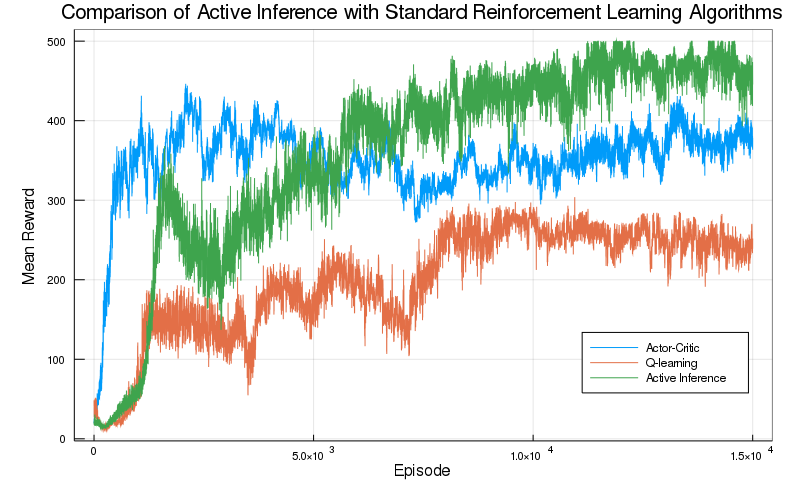
\includegraphics[scale=0.4]{chapter_4_figures/basic_comparison_graph.png}
    \caption{Comparison of the mean reward obtained by the Active Inference agent compared to two reinforcement learning baseline algorithms -- Actor-Critic and Q learning on the CartPole environment. We demonstrate the learning curves over 2000 episodes, averaged over 5 different seeds. 500 is the maximum possible reward. We see that while the vanilla actor critic agent initially learns faster, over a long time horizon, the active inference agent outperforms it -- and both perform better than the vanilla Q learning agent.}
    \label{CartPole Comparison}
\end{figure}

\begin{figure}[H]
\centering
    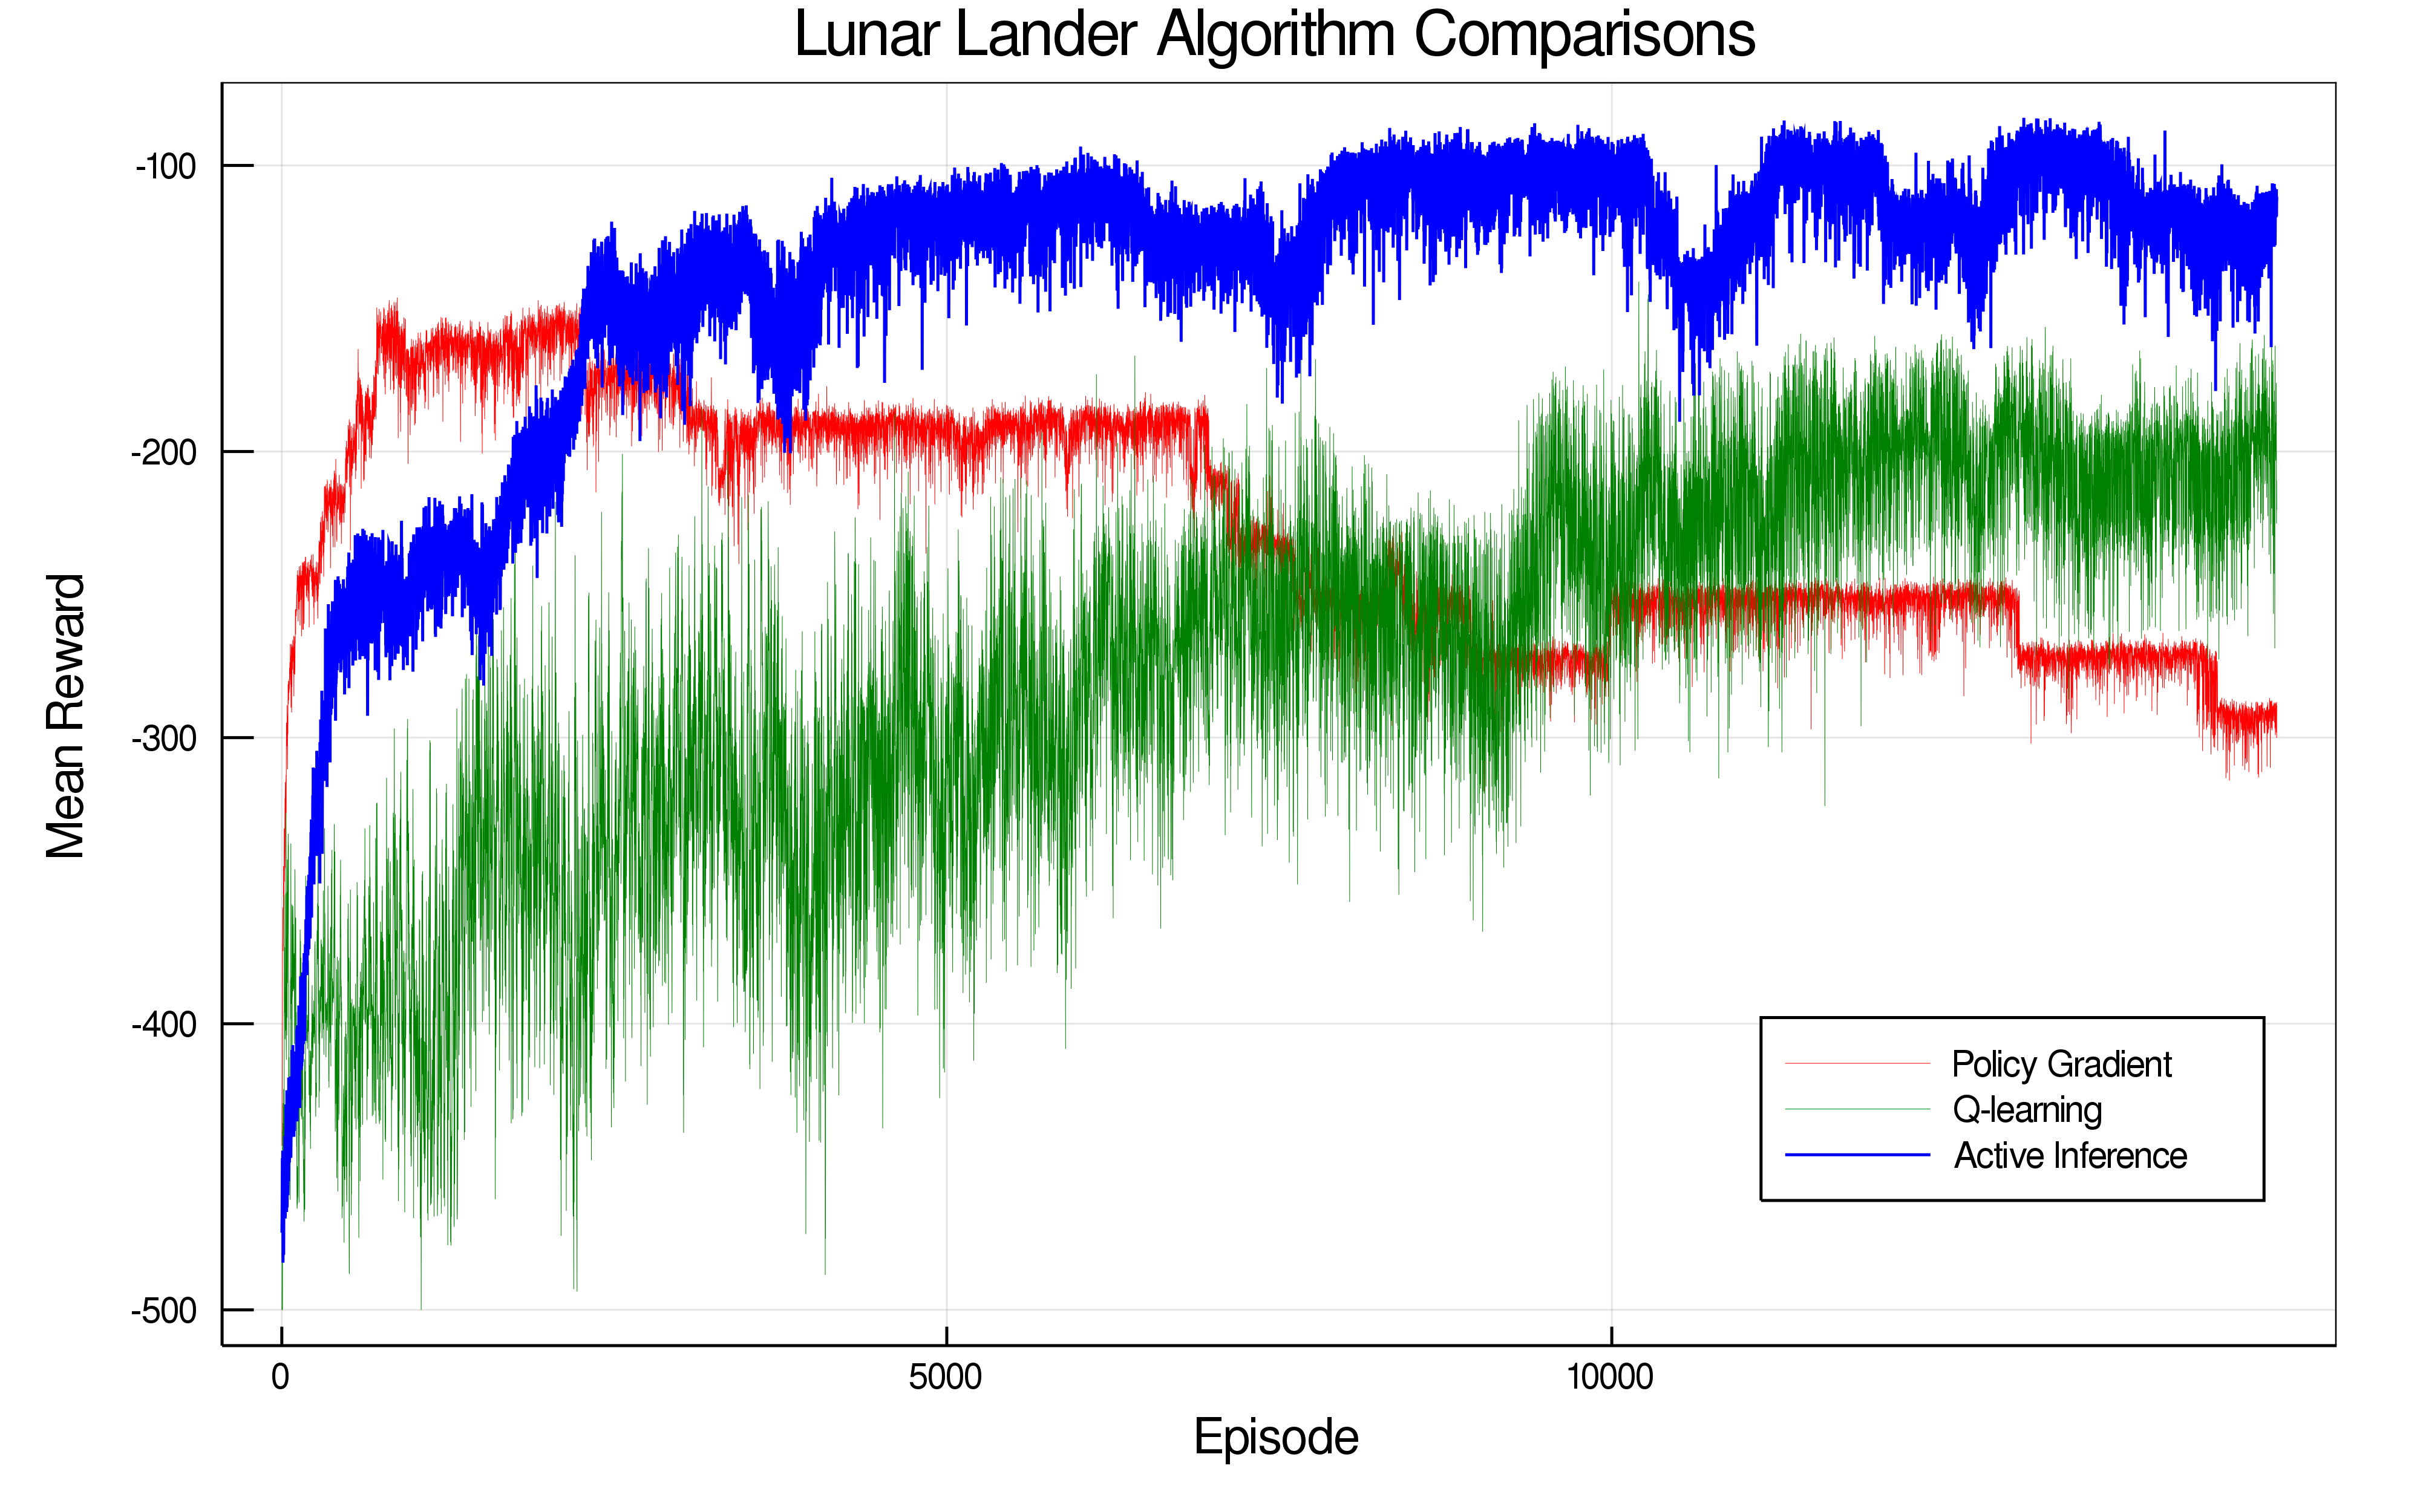
\includegraphics[scale=0.08]{chapter_4_figures/Acrobot_Comparison_Graph.png}
    \caption{Comparison of Active Inference with standard reinforcement learning algorithms on the Acrobot environment. Here we see the learning curves plotted over five seeds over 20000 episodes. The maximum possible reward in this environment was 0, so no agents are optimal. We see again that active inference outperforms the other two methods consistently.}
\end{figure}
\bigskip
\begin{figure}[H]
    \centering
    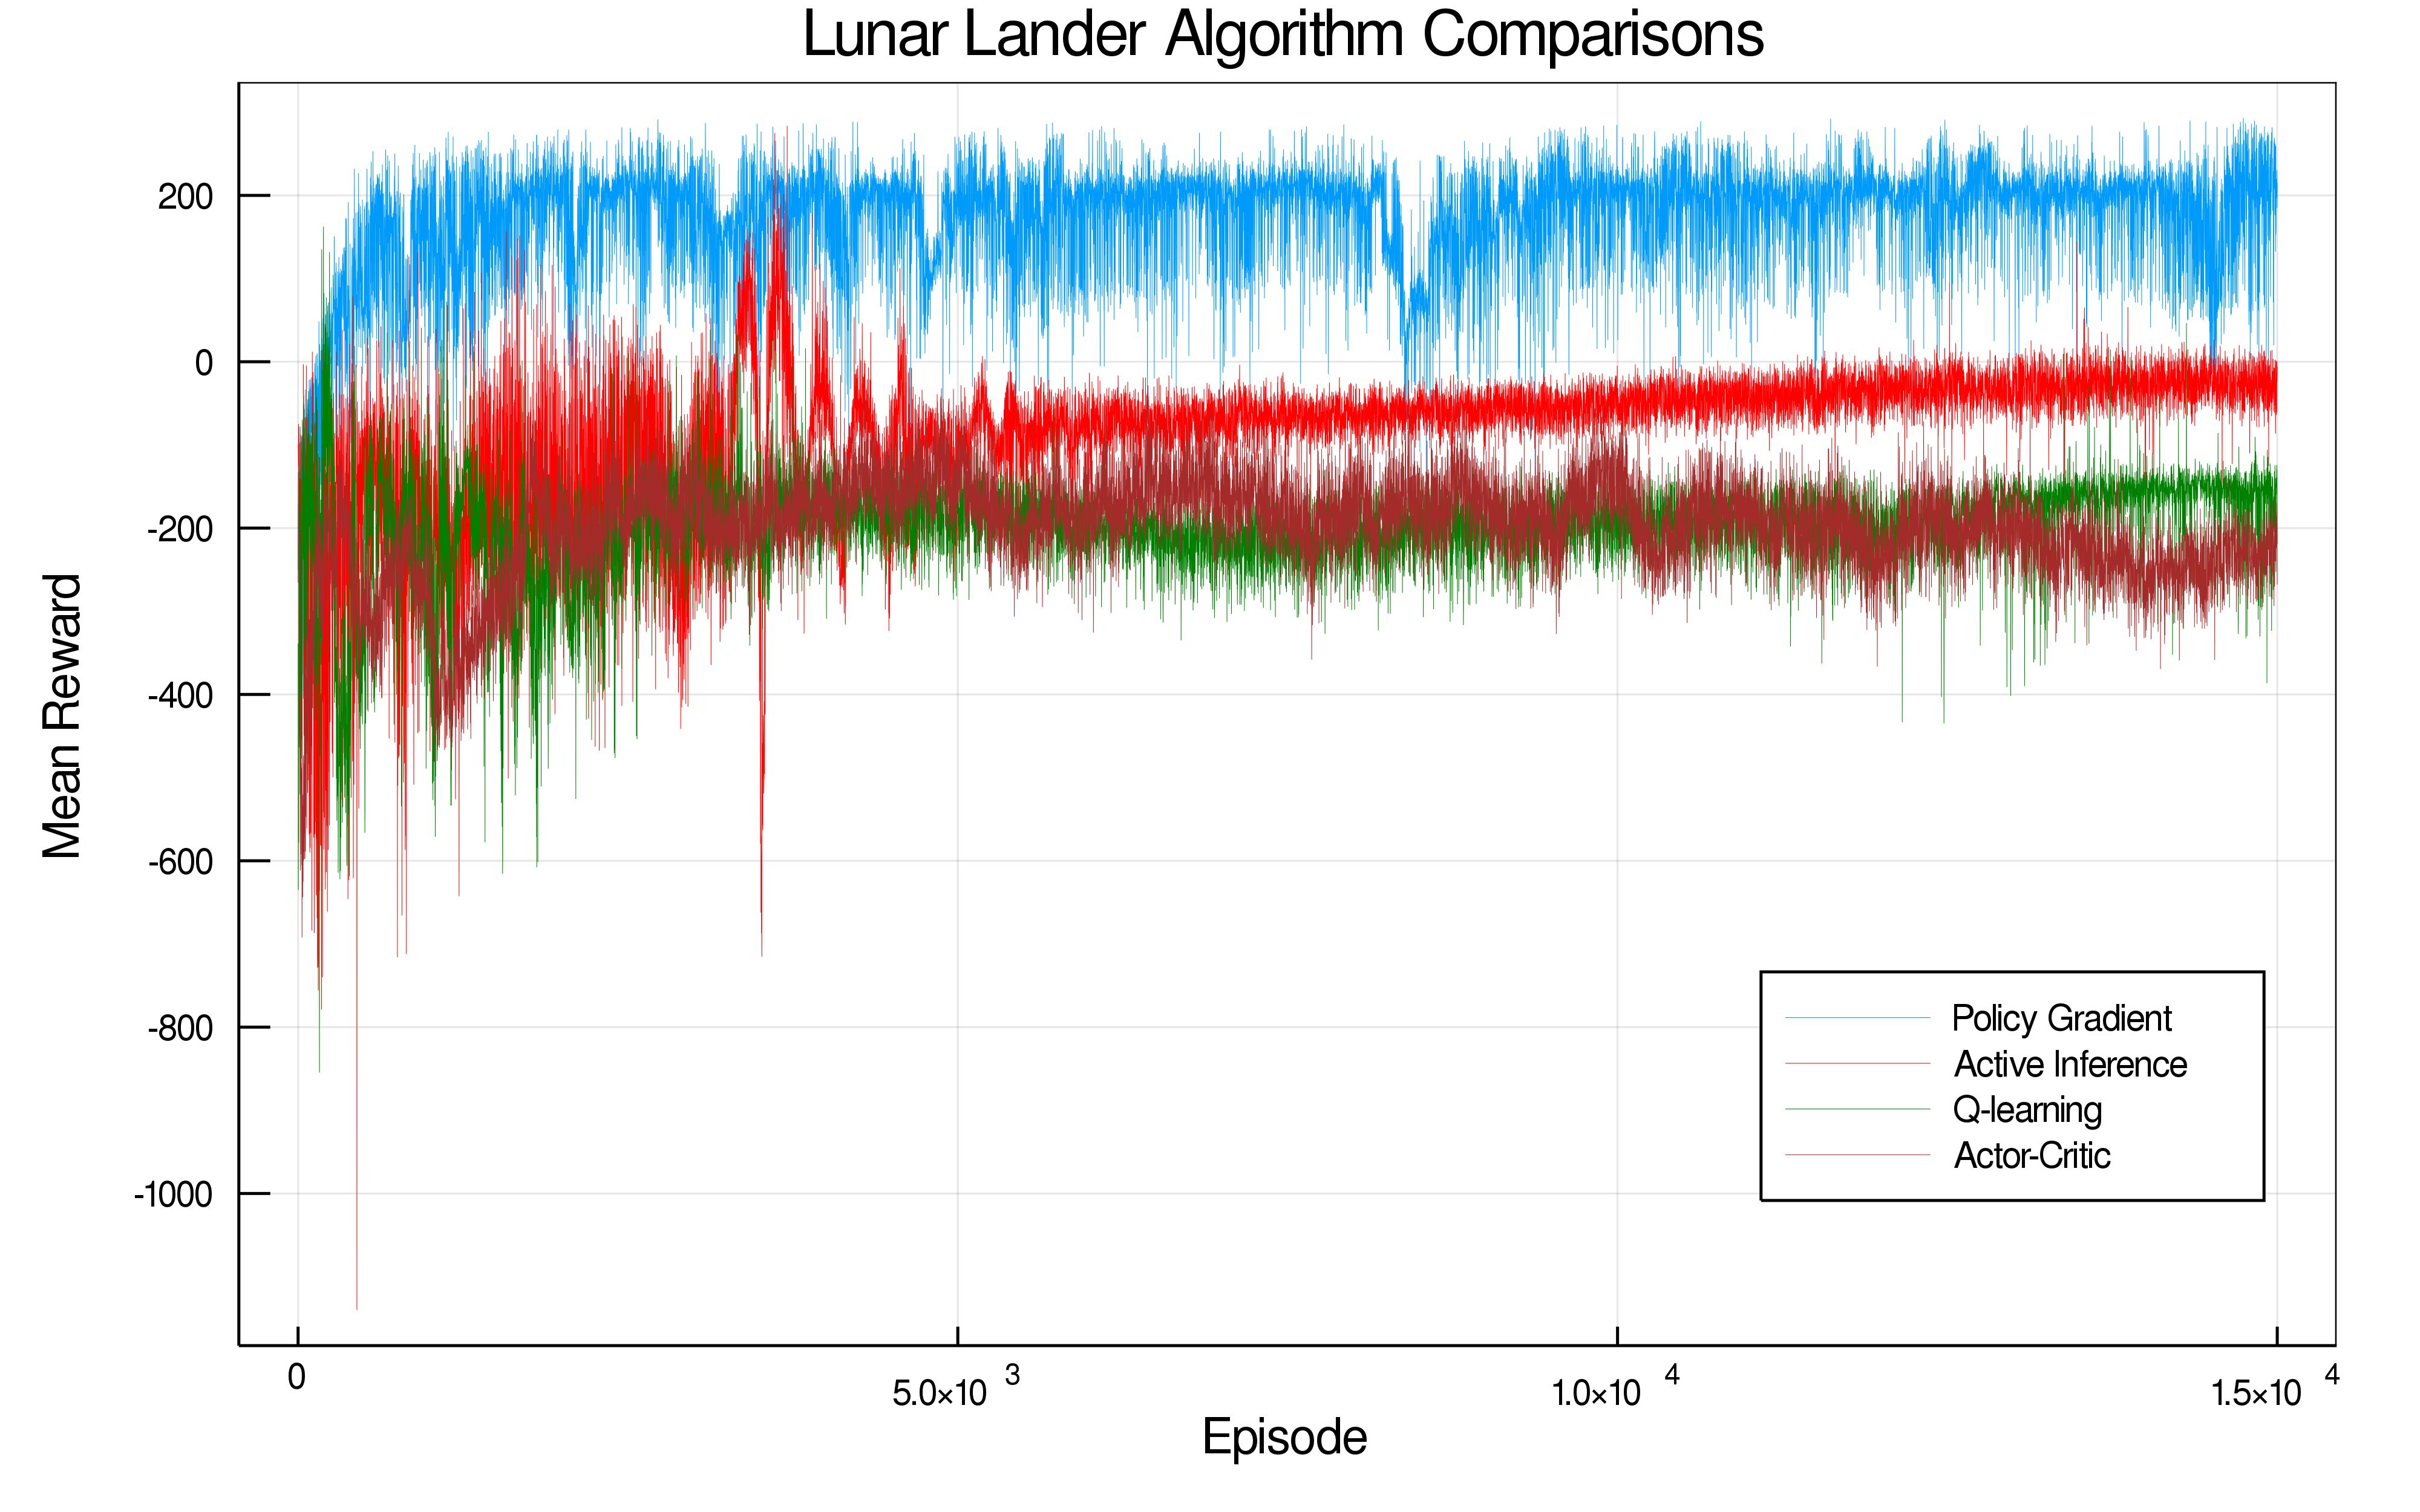
\includegraphics[scale=0.08]{chapter_4_figures/Lunar_Lander_Comparison_Graph.png}
    \caption{Comparison of Active Inference with reinforcement learning algorithms on the Lunar-Lander environment. Learning curves presented over 15000 episodes, averaged over 5 seeds. Here the vanilla policy gradient algorithm strongly outperforms the others, for unclear reasons, although active inference is still comparable with the other standard reinforcement learning algorithms. A score of 200 is optimal.}
\end{figure}

Since the active inference agent possesses several distinct features beyond the standard actor critic architectures, we performed an ablation study to understand whence its boost in performance arose.

\begin{figure}[H]
    \centering
    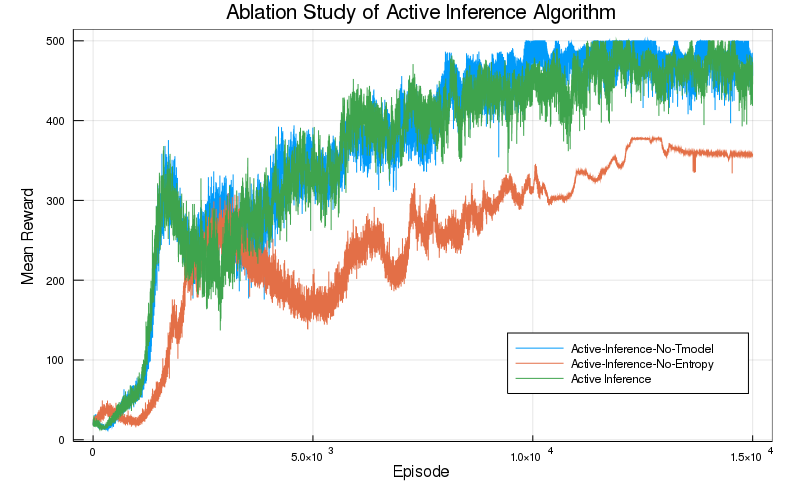
\includegraphics[scale=0.4]{chapter_4_figures/ablation_graph.png}
    \caption{We compare the full Active Inference agent (entropy regularization + transition model) with an Active Inference agent without the transition model, and without both the entropy term and the transition model). We see that while removing the transition model appears to have little effect, removing the entropy regularisation term substantially impairs performance. This may be due to the entropy term aiding in staving off policy collapse.}
    \label{Active Inference Ablation}
\end{figure}

\begin{figure}[H]
    \centering
    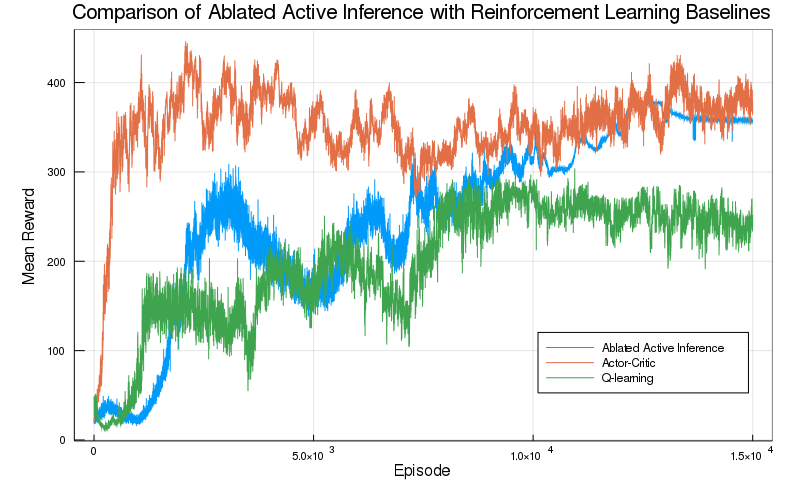
\includegraphics[scale=0.4]{chapter_4_figures/ablation_comparison_graph.png}
    \caption{Comparison of the rewards obtained by the fully ablated Active Inference agent with standard reinforcement-learning baselines of Q-learning and Actor-Critic on the CartPole environment. Learning curves are averaged over 5 seeds. We see that despite being fully ablated, the active inference agent continous to perform comparably with standard reinforcement learning agents.}
    \label{Ablation Comparison}
\end{figure}

 We see that the key factor in the superior performance of the active inference agent is the additional action entropy term that is additionally optimized. This provides additional empirical confirmation to the success of control-as-inference approaches in the reinforcement literature which similarly utilize such an entropy regularisation term. Perhaps surprisingly, we found little effect of the epistemic terms in the EFE on total performance. We hypothesise that this was for two reasons. Firstly, the tasks that were tested possessed a relatively dense reward structure, sufficient to be learned by standard reinforcement learning agents utilizing only random exploration strategies, and thus that more advanced and powerful exploration strategies are likely unnecessary for such tasks. Secondly, the epistemic action term was the information gain between the prior and posterior states, which is effectively a measure of the predictive success of the transition model. Importantly, we found that the transition model very rapidly converged during training, much faster than the policy or value network, and thus that throughout most of the training period, the exploration term was thus negligible.

\subsubsection{Interim Discussion}

In this section, we have demonstrated how active inference approaches can be straightforwardly scaled up by parametrizing the likelihood, inference, and transition distributions with deep neural networks, and then additionally approximating the path integral of the expected free energy with an amortized value network. This is possible because the expected free energy satisfies a similar Bellman-like recursion to the reward in reinforcement learning, because it is factorizable across time into a sum of independent time-steps. Importantly, we have demonstrated that by taking this approach, our active inference agent can handle complex machine learning benchmark tasks just as well as several core deep reinforcement learning approaches, thus rendering it significantly more scalable than previous efforts in the literature which have generally been restricted to small, discrete, and straightforwardly enumerable state spaces.

Moreover, we have shown that our algorithm is competitive, and in some cases superior, to standard baseline reinforcement learning agents on a suite of reinforcement learning benchmark tasks from OpenAI Gym \citep{brockman2016openai}. While our active inference agent performed worse than direct policy gradients on the Lunar-Lander task, we believe this is due to the inaccuracy of the expected-free energy-value-function estimation network, since the policy gradient method used direct and unbiased monte-carlo samples of the reward rather than a bootstrapping estimator. Since the performance of Active Inference, at least in the current incarnation, is sensitive to the successful training of the EFE-network, we believe that improvements here could substantially aid performance. Moreover, it is also possible to forego or curtail the use of the bootstrapping estimator and use the generative model to directly estimate future states and the expected-free energy thereof, at the expense of greater computational cost. We take this approach of using the transition model to generate sample rollouts and using these to compute a Monte-Carlo estimate of the EFE path integral in the next section, where these estimates are used to inform model-predictive planning.

An additional advantage of our approach is that due to having the transition model, it is possible to predict future trajectories and rewards N steps into the future instead of just the next time-step. These trajectories can then be sampled from and used to reduce the variance of the bootstrapping estimator, which should work as long as the transition model is accurate. This $N$ could perhaps even be adaptively updated given the current accuracy of the transition model and the variance of the gradient updates. This is a way of controlling the bias-variance trade-off in the estimator, since the future samples should reduce bias while increasing the variance of the estimate, and also the computational cost for each update. 
\newline

Another important parameter in active inference is the precision \citep*{feldman2010attention,kanai2015cerebral}, which in the discrete-state-space paradigm corresponds to the inverse temperature parameter in the softmax and so controls the stochasticity of action selection \footnote{In the continuous predictive coding paradigm the precision modulates the `importance' of the prediction errors.}. In all simulations reported above we used a fixed precision of 1. However, in the discrete state-space case, the precision is often explicitly optimized against the variational free energy, and the same can be done in our deep active inference algorithm. In fact, the derivatives of the precision parameter can be computed automatically using automatic differentiation. Determining the impact of precision optimization on the performance of these algorithms is a potentially worthwhile avenue for future work. 

While we did not find that using the epistemic reward helped improve performance on our benchmarks, this could be due to the simplicity of the tasks we were trying to solve, for which random exploration is sufficient. In the next section, we demonstrate that the epistemic affordances engendered by the use of the EFE value function prove instrumental in attaining high performance in sparse-reward tasks.

The entropy regularization term which emerges directly from the mathematical formulation of active inference proved to be extremely important, and was often the factor causing the superior performance of our active inference agent to the reinforcement learning baselines. This entropy term is interesting, since it parallels similar developments in reinforcement learning, which have also found that adding an entropy term to the standard sum of discounted returns objective improves performance, policy stability and generalizability \citep*{haarnoja2017reinforcement,haarnoja2018acquiring}. This is of even more interest given that these algorithms can be derived from a similar variational framework which also casts control as inference \citep*{levine2018reinforcement}. Later (in Chapter 5), we discuss in significant detail how such paradigms relate to active inference. Additionally, many of the differences between active inference and the standard policy gradients algorithm -- such as the expectation over the action, and the entropy regularization term  -- have been independently proposed to improve policy gradient and actor critic methods \citep{fujimoto2018addressing}. The fact that these improvements fall naturally out of the active inference framework could suggest that there is deeper significance to the probabilistic inference formulation espoused by active inference. The other key difference between policy gradients and active inference is the optimization of the policy probabilities versus the log policy probabilities, and multiplying by the log of the probabilities of the estimated values, rather than the estimated values directly. It is currently unclear precisely how important these differences are to the performance of the algorithm, and their effect on the numerical stability or conditioning of the respective algorithms, and this is also an important avenue for future research. However, the comparable performance of active inference to actor-critic and policy gradient approaches in our results suggest that the effect of these differences may be minor.

\subsection{Model-based: Reinforcement Learning through Active Inference}

While the last section focused on scaling active inference using model-free reinforcement learning methods, here we focus on scaling active inference in a way inspired by model-based reinforcement learning methods.
Model-based reinforcement learning is perhaps a better fit for the central ideas in the classical active inference. Tabular active inference, after all, is a model-based algorithm which explicitly evaluates and optimizes future plans using explicit models of the environmental dynamics. Moreover, as tabular active inference explicitly replans at every time-step, it can be considered to be a model-predictive control algorithm. In fact, the explicit enumeration and evaluation of every possible policy can perhaps best be thought of as a truly exhaustive planning algorithm.

Similar to our previous approach described earlier, we propose to develop deep active inference methods which utilize deep neural networks to parametrize key distributions from the active inference framework. Specifically, we maintain deep neural network representations of the observation likelihood distribution $p(o_t | x_t)$ as well as the transition model which parametrises the dynamics model of the environment $p(x_t | x_{t-1}, a_{t-1})$. The major difference is how the action policy $q(a_t | x_t)$ is handled. In the previous model-free approach, this distribution was represented as an independent policy neural network which was trained against the action prior which represented the softmax of the expected free energy value function in an actor-critic like fashion. Here, we treat the action posterior as the output of a model-based planning algorithm.

Specifically, and quite elegantly, we can show that under certain conditions of the generative model of the future, that we can derive the optimal plan as a softmax over the expected free energy in the future, (which was merely assumed to be the action prior in the model-free case). Moreover, we then show that this path integral can be approximated by monte-carlo sampling in the form of a model-based planning algorithm which samples and evaluates given potential future trajectories using the transition and reward models possessed by the agent.

\begin{align*}
          \mathcal{\tilde{F}}_{\pi} &= \KL \Big( q(o_t, x_t, \theta , \pi ) \Vert \tilde{p}(o_t, x_t, \theta) \Big) \\
         &= \mathbb{E}_{q(o_t, x_t, \theta ,\pi)}[\log q(o_t, x_t, \theta |\pi) + \log q(\pi) - \log \tilde{p}(o_t, x_t, \theta,  \pi)] \\
         &=  \mathbb{E}_{q(\pi)} \Big[ \mathbb{E}_{q(o_t, x_t, \theta| \pi)}[ \log q(\pi) - [\log \tilde{p}(o_t, x_t, \theta) - \log q(o_t, x_t, \theta |\pi)]\Big] \\
         &= \mathbb{E}_{q(\pi)} \Big[\log q(\pi) - \mathbb{E}_{q(o_t, x_t, \theta| \pi)}[\log \tilde{p}(o_t, x_t, \theta) - \log q(o_t, x_t, \theta |\pi)]\Big] \\
         &= \mathbb{E}_{q(\pi)} \Big[\log q(\pi) - \big[-\mathbb{E}_{q(o_t, x_t, \theta| \pi)}[\log q(o_t, x_t, \theta |\pi) - \log \tilde{p}(o_t, x_t, \theta)]\big]\Big] \\
         &= \mathbb{E}_{q(\pi)} \Big[\log q(\pi) - \log e^{- \big[-\mathbb{E}_{q(o_t, x_t, \theta| \pi)}[\log q(o_t, x_t, \theta |\pi) - \log \tilde{p}(o_t, x_t, \theta)]\big]} \Big] \\
         &= \mathbb{E}_{q(\pi)} \Big[\log q(\pi) - \log e^{-\KL \big( q(o_t, x_t, \theta | \pi) \Vert \tilde{p}(o_t, x_t, \theta) \big)}\Big] \\
         &= \KL \Big( q(\pi)  \Vert  e^{- \KL \big( q(o_t, x_t, \theta | \pi) \Vert \tilde{p}(o_t, x_t, \theta) \big)} \Big) \\
         &= \KL \Big( q(\pi)  \Vert  e^{-\mathcal{\tilde{F}_{\pi}}} \Big) \numberthis
\end{align*}

It is important to note that here we do not use the expected free energy as our objective, unlike in standard active inference. Instead, we use the recently introduced objective: the free energy of the expected future (FEEF). This objective maintains the exploratory information gain terms of the traditional expected free energy while possessing a clear mathematical origin with strong intuitive grounding. Specifically, the FEEF can be defined as,

\begin{align*}
    \mathbb{FEEF} = \tilde{\mathcal{F}}_\pi &= \KL[q(o_t, x_t, \theta | \pi) || \tilde{p}(o_t, x_t, \theta) \\
    &\approx \underbrace{\mathbb{E}_q(x_t | \pi)\KL [q(o_t | x_t) || \tilde{p}(o_t)]}_{Extrinsic Value} - \underbrace{\mathbb{E}_{q(o_t; \theta)}\KL[q(x_t | o_t, \theta) || q(x_t)]}_{\text{State Information Gain}} \\ &- \underbrace{\KL [q(\theta | x_t) || q(\theta)]}_{\text{Parameter Information Gain}} \numberthis
    &
\end{align*}
Where we can see that the FEEF can be split into approximately three terms -- the likelihood divergence term which measures how much the expected observations diverge from the desired observations, and which effectively encodes reward or utility seeking behaviour, and an information gain term to be maximized which induces exploratory, uncertainty reducing behaviour. Since the FEEF objective includes both latent states $x$ and parameters $\theta$, we actually obtain two separate information gain terms, one for the states and one for the parameters. The core finding and argument of this part of the chapter, and an example of what the theory of active inference can bring to contemporary deep reinforcement learning, is that the exploratory information-seeking terms furnished by active inference objectives such as the expected free energy, or free energy of the expected future, by inducing \emph{purposeful} and \emph{goal-directed} exploratory behaviour, they can outperform traditional random exploration on a number of challenging reinforcement learning tasks, and their advantages become especially apparent in the case of sparse rewards where random exploration is often simply insufficient to find any good solutions in a reasonable time. Moreover, recent work in the literature, which utilizes exploratory objectives, but in a first exploratory, and then exploitatory phase, we argue that it is necessary to combine the two objectives to be jointly optimized. In this way the agent is furnished with a desire for \emph{goal directed exploration}. It is not rewarded simply for reducing any uncertainty, but only uncertainty that also exists in rewarding regions in the state-space. In this way, agents explore precisely only as much as needed, thus providing a step towards a practical solution to the exploration-exploitation tradeoff.

\subsubsection{Model} 

As in previous work, we extended active inference by using deep neural networks to parametrize key densities. Our model utilized a neural network transition model to model the distribution $p(x_t | x_{t-1, a_{t-1})})$. Since the FEEF objective requires the evaluation of an information gain term over the parameters (denoted $\theta$) of the transition model, we maintained an approximate distribution over the parameters $\theta$ using an ensemble of transition models with independently initialized parameters, and trained on different batches from the replay buffer. This ensemble approach has been found to be widely useful in model-based reinforcement learning and to offer a superior representation of the true posterior over the parameters than competing methods such as Bayesian neural networks. Importantly, utilizing an explicit ensemble of transition models allows the estimated posterior over the parameters to be multimodal, as opposed to the unimodal Gaussian assumption implicit in the Bayesian neural networks approach \citep{tran2018Bayesian,gal2016improving}. Moreover, an ensemble of models has been found empirically to help avoid overfitting in low-data regimes, which are also when the advantages of model-based reinforcement learning are most apparent.
Each element of the transition model ensemble was implemented as an independent neural network with two hidden layers with 400 neurons each. The networks used the swish activation function. The transition networks predicted the \emph{difference} in the next state \citep{shyam_model-based_2019} instead of the next state, as this has been found to help capture environmental dynamics more accurately in practice.
Since we are evaluating future simulated rollouts, we cannot simply rely on environmentally provided `true rewards'. While many methods in the literature assume the existence of a known reward function which can be queried even for counterfactual or simulated trajectories \citep{chua_deep_2018,hafner2018learning}, we do not, as such a reward oracle is unrealistic in many if not most situations. Instead, we learnt a reward model based upon previous interactions with the real environment, and then used the reward model to score proposed trajectories. The reward model was parametrised by a two layer multi-layer perceptron network with 400 units in the hidden layer and a relu activation function. The reward model was trained on a mean-square error loss between actually observed rewards for a given state, and the reward predicted by the reward model.
Importantly, the FEEF objective defines the extrinsic reward to be the KL divergence between the observation likelihood and the desired observation distribution. Since our model was situated purely in an MDP setting with fully observed state, the only observation was the reward, and thus the reward model doubled as the likelihood model. We set the desired reward observations to be a Gaussian distribution with a variance of 1 centred at the maximum possible reward for the environment. Since we interpret the predictions of the reward model as representing the mean of a Gaussian distribution, we can analytically calculate the KL divergence term. This allowed us to straightforwardly compute and optimize the reward maximization part of the FEEF objective.
Similarly, to evaluate the information gain terms of the FEEF objective, we can rewrite it in a more tractable way,

\begin{align*}
        & \E_{q(x_t | \theta)}\KL \big(q(\theta | x_t) \Vert q(\theta) \big) \\
        &= \E_{q(x_t | \theta)q(\theta | rs)}\big [ \log q(\theta | x_t) - \log q(\theta) \big] \\
        &= \E_{q(x_t, \theta)}\big [ \log q(x_t | \theta) + \log q(\theta) - \log q(x_t) - \log q(\theta) \big] \\
        &= \E_{q(x_t, \theta)}\big [ \log q(x_t | \theta)  - \log q(x_t) \big] \\
        &= \E_{q(\theta)q(x_t | \theta)}\big [\log q(x_t | \theta) \big]  -\E_{q(\theta)q(x_t|\theta)} \big[ \log \E_{q(\theta)} q(x_t | \theta) \big] \\
        &= -\E_{q(\theta)}\mathcal{H}\big[ q(x_t | \theta) \big] + \mathcal{H} \big[ \E_{q(\theta)}q(x_t | \theta) \big] \numberthis
\end{align*}

In effect, the parameter information gain term decomposes into an entropy of the average state minus the average of the entropy. The average of the entropy can be computed semi-analytically since each transition model ensemble models a Gaussian distribution, which has a known and analytically calculable entropy. Then, the average can simply be performed by directly averaging the entropies of each member of the ensemble together. The entropy of the average term is more difficult, since the average of many different Gaussian distributions is not necessarily Gaussian. As such we approximate it with a nearest neighbour entropy approximation \citep{mirchev_approximate_2018} which we found worked well in practice.

To train the model, we optimized the reward and transition models on data taken from a replay buffer. They were trained with stochastic gradient descent on their respective loss functions using a negative log likelihood loss. We cold-started the training of the agent at the end of every episode, as we found that this led to more consistent behaviour and performance. We initialized each episode with a dataset $\mathcal{D}$ taken from an agent with a random policy, to ensure some degree of transition and reward model accuracy before beginning with the model-based planning.

To compute actions we used a model-based planner (CEM) \citep{rubinstein1997optimization} within the model-predictive control paradigm. The CEM planning algorithm generates and evaluates the reward of a large number of action trajectories, then takes the mean and variance of some elite set of actions (usually the top 10) of the actions and restarts the evaluation using actions sampled from a Gaussian distribution with this mean and variance. For every timestep, a 30 step planning horizon was used resulting in a 30-step action plan, of which the first action was executed. In accordance with model-predictive control, we replan at each step. For the CEM algorithm, we used 700 candidate action sequences to be evaluated in each iteration, for 7 iterations. To train the transition and reward models we used the ADAM optimizer with a learning rate of 1e-4 and trained for 100 epochs.

\begin{algorithm}[H]
\label{algo:exps}
\SetAlgoLined
   \DontPrintSemicolon
   \textbf{Input:} Planning horizon $H$ | Optimisation iterations $I$ | Number of candidate policies $J$ | Current state $s_t$ | Likelihood $p(o_\tau|s_\tau)$ |  Transition distribution $p(s_\tau|s_{\tau-1}, \theta, \pi)$ | Parameter distribution $P(\theta)$ | Global prior $\tilde{p}(o_\tau)$
   \BlankLine
   Initialize factorized belief over action sequences $q(\pi) \leftarrow \mathcal{N}(0,\mathbb{I})$.
   
   \For{$\mathrm{optimisation \ iteration} \ i = 1...I$}{
      Sample $J$ candidate policies from $q(\pi)$ \;
      \For{$\mathrm{candidate \ policy} \ j = 1...J$}{
      $\pi^{(j)} \sim q(\pi)$ \;
      $-\mathcal{\tilde{F}}_{\pi}^j = 0$ \;
      \For{$\tau = t...t+H$}{
         $q(s_\tau| s_{\tau-1}, \theta, \pi^{(j)}) = \E_{q(s_{\tau-1}|\theta, \pi^{(j)})} \big[p(s_\tau|s_{\tau-1}, \theta, \pi^{(j)})\big]$ \;
         $q(o_\tau| s_\tau, \theta, \pi^{(j)}) = \E_{q(s_\tau|\theta, \pi^{(j)})} \big[p(o_\tau|s_\tau)\big]$ \;
         $-\mathcal{\tilde{F}}_{\pi}^j \leftarrow -\mathcal{\tilde{F}}_{\pi}^j + E_{q(s_\tau,\theta | \pi^{(j)})} \big[ \KL \big( q(o_\tau | s_\tau, \theta, \pi^{(j)}) \Vert \tilde{p}(o_\tau) \big) \big]  
          +\mathbf{H}[q(s_{\tau}| s_{\tau-1}, \theta, \pi^{(j)})] - \mathbb{E}_{q(\theta)}\big[\mathbf{H}[q(s_{\tau}| s_{\tau-1}, \pi^{(j)}, \theta)]\big]$
      }
   }
   $q(\pi) \leftarrow \mathrm{refit}(-\mathcal{\tilde{F}}_{\pi}^j)$
}
\textbf{return} $q(\pi)$
\caption{Inference of $q(\pi)$}
\end{algorithm}

\subsubsection{Results}

We tested the performance of our algorithm against strong model-free and model-based baselines on a number of challenging control tasks \footnote{Different tasks are utilized in this section compared to the previous one because here we are dealing with continuous actions while in the previous section we dealt only with learning discrete-action controllers.}. We utilized first the mountain-car task from OpenAI Gym, which requires the agent to steer a car on a 1D line to a goal. This task is difficult because the agent must first move the car away from the goal up a hill, to build up momentum to be able to get over the larger hill. This poses a difficult exploration problem which purely random exploration agents struggle to solve. By contrast, our agent can solve this task instantaneously, within only a single episode, due to its goal directed exploration.

\begin{figure}[h]
   \centering 
      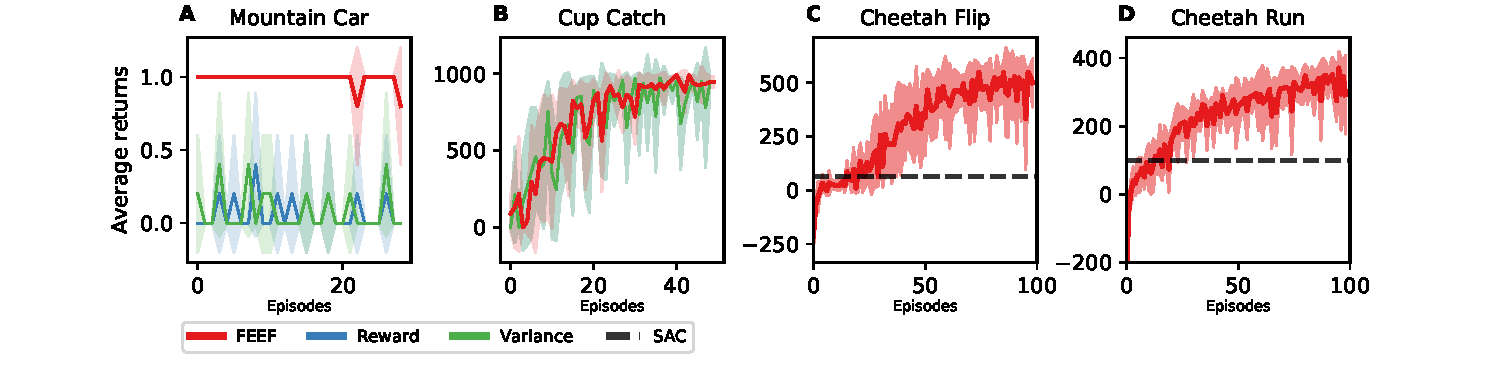
\includegraphics[width=15cm]{chapter_4_figures/RLAI_performance.pdf}
      \caption{\textbf{(A) Mountain Car:} Average return after each episode on the sparse-reward Mountain Car task. Our algorithm achieves optimal performance in a single trial. \textbf{(B) Cup Catch:} Average return after each episode on the sparse-reward Cup Catch task. Here, results amongst algorithms are similar, with all agents reaching asymptotic performance in around 20 episodes. \textbf{(C \& D) Half Cheetah:} Average return after each episode on the well-shaped Half Cheetah environment, for the running and flipping tasks, respectively. We compare our results to the average performance of SAC after 100 episodes learning, demonstrating our algorithm can perform successfully in environments which do not require directed exploration. Each line is the mean of 5 seeds and filled regions show +/- standard deviation.}
   \end{figure}

Since the mountain car environment possesses only a two dimensional state space, we can explicitly plot and compare the degree of the space covered by the active inference agent vs the greedy reward maximizing reinforcement learning agent.

\begin{figure}[h]
   \centering 
   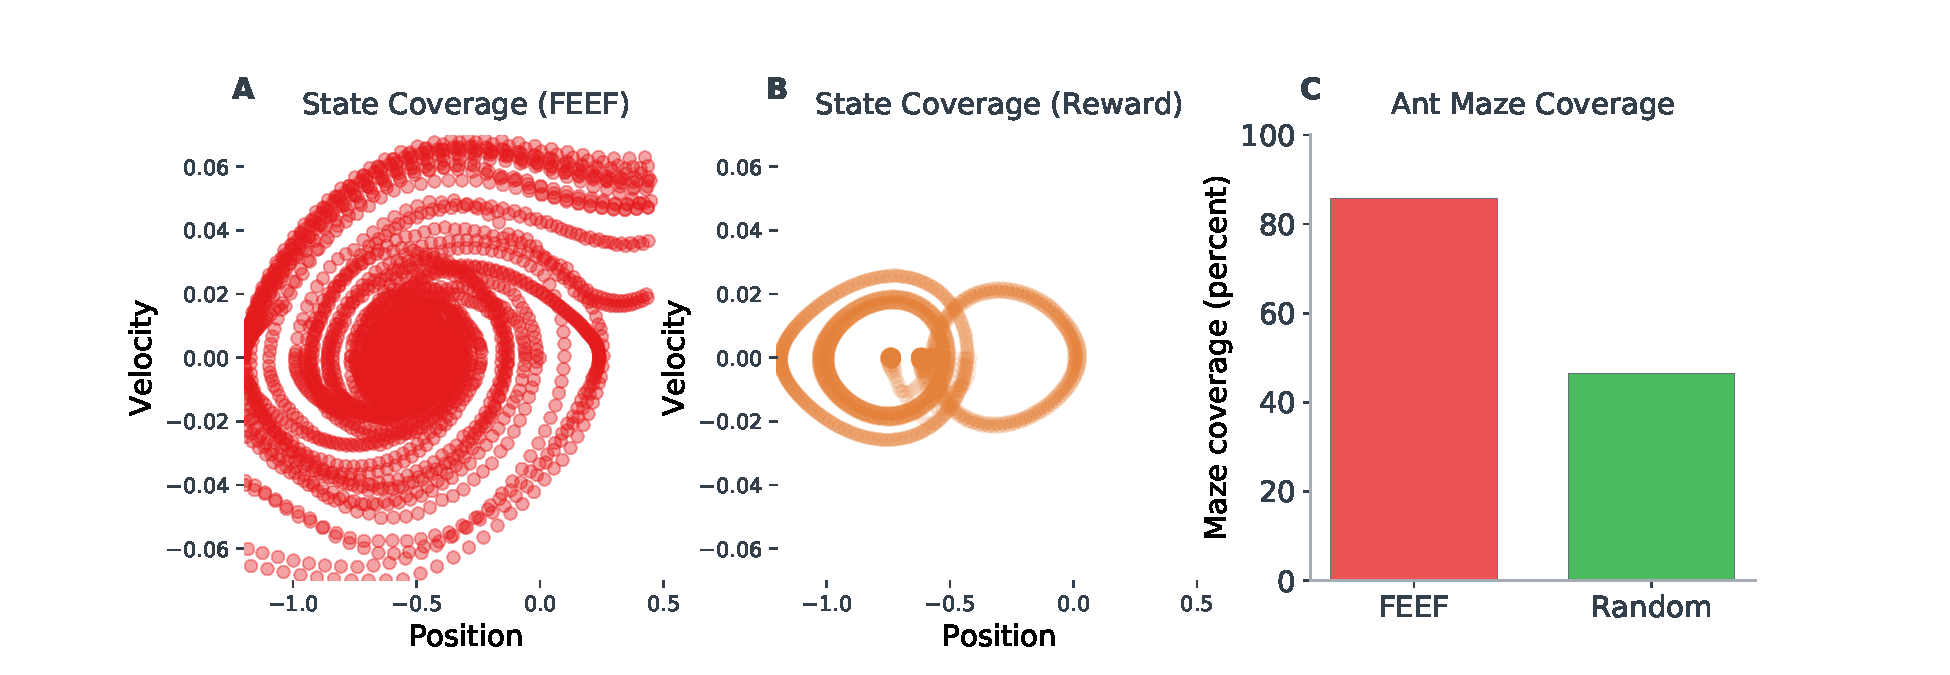
\includegraphics[width=12cm, height=4cm]{chapter_4_figures/RLAI_figure_two.pdf}
\caption{\textbf{(A \& B) Mountain Car state space coverage}: We plot the points in state-space visited by two agents - one that minimizes the free energy of the expected future (FEEF) and one that maximises reward. The plots are from 20 episodes and show that the FEEF agent searches almost the entirety of state space, while the reward agent is confined to a region that can be reached with random actions. \textbf{(C) Ant Maze Coverage}: We plot the percentage of the maze covered after 35 episodes, comparing the FEEF agent to an agent acting randomly. These results are the average of 4 seeds.}
\end{figure}


We thus see that the exploratory drives inherent in the active inference agent propel it to explore a significantly larger fraction of the state-space than the reward maximizing agent, and it is this exploration which allows it to stumble upon the goal and thus rapidly learn to solve the task. By contrast, the random exploration reward-maximizing agent is unable to escape the local minimum at its start location by a purely random walk, since to do so requires too many correct moves in a sequence than can be generated within a reasonable time.
We also tested our agent on sparse reward versions of two challenging control tasks. In the first task, Cup Catch, the agent must actuate a cup to catch a ball thrown at it. The agent receives a reward of 1 if it catches the ball, and a reward of 0 if it does not. Similarly, in the Half-Cheetah environment, the agent takes control of the limbs of a running planar cheetah in a semi-realistic physics simulation. Its goal is to maximize the velocity at which the cheetah moves forward, ideally by running. We also experimented with a no-reward environment to test the pure exploration capabilities of our agent. For this we utilized the ant-maze environment in which the agent must actuate an ant-like robot in order to explore as much of a maze as possible. The agent receives no extrinsic rewards at any point in this task.

Overall, we see that the active inference and reward maximization agent performs similarly in the cup-catch environment. We hypothesise that this is because, even with the sparse reward, the reward is easy enough to obtain even with purely random behaviour. Similarly, on the half-cheetah benchmark, our model performs significantly better than the model-free SAC agent, due to the superior sample efficiency of model-based over model-free methods, however it also does not show much significant improvement compared to reward maximizing model-based baselines. However in the ant-maze environment, our agent evinces significantly more exploration capacity and explores a substantially larger proportion of the total state space than any other agent, once again demonstrating its superior exploratory capabilities.

\subsubsection{Interim Discussion}

So far, in this chapter, we have applied an active inference perspective to reinforcement learning and recast the traditional RL objective into a more active-inference-inspired one; reformulating the reward maximization objective as that as minimizing the divergence between predicted and desired probabilistic futures. From this starting point, we can derive a novel algorithm that exhibits high performance as well as robustness, flexibility, and sample efficiency in a number of environments that are known to be exceptionally challenging for traditional reinforcement learning methods, while also performing comparably in environments where standard RL methods do well.

We believe that through these two studies, we have convincingly demonstrated that active inference approaches can be successfully scaled to levels equal to contemporary reinforcement learning methods in both model-free and model-based paradigms. Moreover, we hope to have shown some ways in which the integration of active inference and reinforcement learning can provide novel and useful perspectives to inform and inspire work in the deep reinforcement learning community. We demonstrate that the exploration-inducing properties of active inference objective functionals such as the Expected Free Energy and the Free Energy of the Expected Future are highly beneficial especially in more challenging tasks with sparse or no rewards, while also performing comparably to pure reward maximization approaches on dense reward tasks that can be solved with purely random exploration. Moreover, combining both exploratory and reward maximizing terms in a single objective function and jointly optimizing them is crucial to derive algorithms which can simply learn to solve a task without separate exploratory and exploitatory phases as in much of the literature \citep{shyam_model-based_2019}, although the idea of inducing exploration by optimizing an epistemic term \citep{oudeyer2009intrinsic,schmidhuber2007simple,pathak2017curiosity} has been applied previously in reinforcement learning, and that can be competitive directly with both purely exploratory and purely exploitatory tasks in the regions where each of these methods excel. 

An additional idea, inspired by active inference, which could inform reinforcement learning perspective is the idea of representing preferences, instead of scalar reward values, as a distribution over observations. We believe that this modelling choice could enable greater flexibility in learning non-scalar, non-monotonic reward functions, as well as providing a natural, Bayesian framework for handling the case of unknown, uncertain, or nonstationary reward distributions. We believe that in many naturalistic settings, especially for biological organisms, rewards are not simply given a-priori by some known oracle, but are task-dependent, contingent, often highly uncertain, and nonstationary. Active inference provides a straightforward Bayesian account to handle precisely such conditions. Although in this work, and in much of the literature, we instead take extremely simplifying assumptions such as $\tilde{p}(o) = exp(-r(o))$ to make active inference as close as possible to reinforcement learning, future work should instead head in the opposite direction and try to deliberately explore the regions where active inference approaches offer greater flexibility than the traditional reinforcement learning paradigm, and thus demonstrate the advantages of active inference approaches there.


\subsection{Related Work}

%Ueltzhoffer (2018), to our knowledge, is the first paper to propose approximating the observation and transition models with deep neural networks.  They use single layer tanh networks with sixteen neurons which outputs the mean and variance of a diagonal conditional Gaussian.  They used this model to solve the Mountain-Car problem from OpenAI gym.  A key difference of this work is how they represented action.  They computed continuous actions in a manner that required them to know the partial derivatives of the sensations given the action, which meant propagating throught he environmental dynamics, which are unknown.  Due to this they had to use a black box evolutionary optimizer to optimize their models, which is substantially more sample-inefficient.  In our model we do not use this approach, but instead use a learned amortized inference distribution $Q(a|x)$ and minimize this using a variational approach on the divergence with the approximated true posterior of the value function $p(a|x)$,which is learned through a bootstrapping estimation procedure.  Due to this our method is end-to-end differentiable and all networks can be trained through gradient descent on the variational free energy.While this paper was in preparation, a paper by Catal et al. (2019) came out along similar lines. They also parametrized the observation and transition models with deep neural networks, and they used a ”habit” policy to approximate the expected free energy, analogously to Q learning in reinforcement learning. However, they only applied their model to the Mountain-Car task and also did not derive the full variational derivation of the KL divergence of the action model and the action posterior, but instead used their habit policy or EFE-approximating network to select actions directly through a softmax choice rule. Instead we maintain a separate policy network which adheres more closely to the full free energy derivation and also solve significantly more complex tasks than the Mountain-Car

Before our work in deep active inference there was a small amount of prior work which is important to review. The seminal paper which began this field is \emph{Deep Active Inference} \citep{ueltzhoffer_deep_2018}, which initiated the idea of using deep neural networks to approximate key densities within the active inference paradigm. This paper uses small neural networks to parametrise the transition dynamics and likelihood in active inference, and uses genetic algorithms to directly optimize a policy module of the expected free energy in a black-box fashion. This is because, under their problem setup, the expected free energy depends on the environmental dynamics and is thus nondifferentiable, assuming the environment itself is unknown. They produced a simple agent which can learn to solve the mountain car problem from OpenAI gym after many iterations. This paper was my inspiration to dive deeper into trying to understand the commonalities and differences between deep active inference and deep reinforcement learning.

Another piece of work, arising contemporaneously with my own initial work \citep{millidge2019combining,millidge_deep_2019}, was that by \citet{catal_Bayesian_2019}. They also parametrised the likelihood and transition dynamics using deep neural networks, and additionally explicitly utilized an expected free energy value function. However, instead of directly solving the sparse-reward challenge implicit in the mountain-car environment they tested their agent in, they instead constructed a hand-crafted `state-prior' generated from expert-rollouts which already directly solved the task, thus providing an effectively dense reward signal for this sparse reward problem.

Some other related work is that of \citet{cullen2018active} who also applied active inference to more complex non-toy environments. They trained an active inference agent to play a subset of DOOM -- the `take-cover' environment in OpenAI Gym. However, they still fundamentally utilised the discrete-state-space active inference formulation by discretising the continuous DOOM environment into 8 discrete states using the Harris Corner detection algorithm, and then applying discrete-state active inference onto the discrete states. 

Just after my initial work came similar work by \citet{tschantz_scaling_2019}, who instead applied active inference in a model-based fashion. Their model parametrises the transition dynamics using a deep neural network, and then uses model based planning (using the CEM algorithm) to optimize the expected free energy over time. We jointly extended their model in \citet{tschantz2020reinforcement} to investigate explicitly the exploratory effects of the EFE or FEEF objective, and whether such methods can be further scaled through learning the transition and reward model.

After our work, several recent approaches have scaled active inference further. \citet{ccatal2020learning}, situate deep active inference within a purely POMDP setting, using a VAE encoder and decoder to parametrize the likelihood and state-posterior mappings, and then explicitly compute an action search tree using their transition model to approximate the path integral over the expected free energy through time. Similarly, \citet{fountas2020deep}, also explicitly compute a model-based EFE search tree in their tasks, while simultaneously approximating the output of the action planner with a model-free `habitual' policy network.

\subsection{Iterative and Amortised Inference}

Now that we firmly understand the notion of implementing control as an inference procedure, it is worth recapping a fundamental distinction between two different \emph{types} of inference, which are important and implicit in the literature, but rarely well explained. The crucial distinction is between what we call \emph{iterative} and \emph{amortised} inference. Iterative inference is the kind that arises directly from a naive application of Bayes Rule, and was the standard inference approach used until the rise of deep learning very recently \citep{wainwright2008graphical,jordan1998introduction,beal2003variational}. Almost all `classical' variational or Bayesian inference methods are iterative. Amortised inference only became prominent with the advent of the variational autoencoder \citep{kingma_auto-encoding_2013}, but has since become the dominant approach, especially within machine learning. The key distinction is that iterative inference directly optimizes the \emph{parameters} of the variational distribution. For instance, suppose we assume our variational distribution is Gaussian, than iterative inference tries to optimize the means and variance $\phi = \{\mu, \sigma \}$ of this Gaussian to fit some datapoint. This is what is implied by the standard reading of the ELBO or variational free energy equation \citep{hinton1994autoencoders,beal2003variational}.
\begin{align*}
    Iterative = \underset{\phi}{argmax} \, \, \mathbb{E}_{q(x; \phi)}[\ln q(x;\phi) - \ln p(o,x)] \numberthis
\end{align*}

Amortised inference, by contrast, does not \emph{directly} optimize the parameters of the variational distribution. Rather, it \emph{learns} the parameters of a function that \emph{maps data to parameters of the variational distribution}. Effectively, the variational parameters themselves are never optimized directly, they are simply spit out of the amortised function $f$, which is then learned. $\phi = f_\psi(D)$. Rather, it is the parameters of this amortisation function $f_\psi$ that are learned. Importantly, these functions are optimized not just against a single data-point but across the whole dataset $DR$. Once learned, the amortisation function $f$ can be quickly used to compute estimated variational parameters $\hat{\phi}$ for \emph{any} data-point, thus \emph{amortising} the cost of inference across the whole dataset. By contrast, iterative inference must start from scratch from each individual data-point given and optimize the variational parameters afresh. While it is often written the same way, to make the notation very explicit, we write the amortisation objective to be optimized as,

\begin{align*}
    Amortised = \underset{\psi}{argmax} \, \, \mathbb{E}_{p(D)}\Big[ \mathbb{E}_{q(x; \hat{\phi} = f_\psi(D))}[\ln q(x; \hat{\phi} = f_\psi(D)) - \ln p(o,x)] \Big] \numberthis
\end{align*}

The reason that amortised inference has risen to such popularity and ubiquity lately is due to the fact that the amortisation function $f_\psi$ is straightforward to implement as a deep neural network, where $\psi$ are the neural network weights which can be trained by a gradient descent on the ELBO or variational free energy. For instance, in a variational autoencoder, $f_\psi$ is effectively implemented by the encoder, which maps the data directly to the variational parameters (the mean and variance of the Gaussian). The iterative approach, by contrast, would forego the encoder and run gradient descent directly on the mean and variance themselves for each data-points. We thus see why amortised methods are preferred. The amortised method can infer the mean and variance quickly, in one feedforward pass of the network, while gradient descent training is split over an entire dataset. By contrast, the iterative approach would require a gradient descent for every inference that the network wishes to make. Importantly, however, the variational parameters found by the amortised methods are in general worse estimates than those found by iterative inference. This is simply because the iterative inference method optimizes the parameters afresh with each data-point, while amortised inference must try to estimate them given a general function which must work for every datapoint. Thus the amortisation function $f_\psi$ must generalize in a way that iterative methods do not have to, and thus any generalization error will cause the amortised method to perform worse. This difference in performance is called the \emph{amortisation gap}. 

Interestingly, it has recently been shown \citep{marino2018iterative}, that you can gain performance improvements by \emph{combining} iterative and amortised inference together. For instance, in a variational autoencoder, if you first perform the amortised mapping to obtain initial estimates of the variational parameters $\phi$ but then run several iterative descent steps directly on your initial estimates of the parameters, this can improve the inference accuracy and reduce the amortisation gap compared to the pure amortisation approach with only a relatively small computational penalty for each inference.

Given that we know we can understand control problems in terms of inference, it is also interesting to consider whether the type of inference applied in control as inference can be best understood as iterative or amortised inference. Indeed, we argue that this distinction between iterative and amortised inference maps rather cleanly (although not perfectly) to the distinction between model-based and model-free reinforcement learning. Where model-free RL can be thought of as amortised inference and model-based as iterative inference. The reasoning here is straightforward but requires some subtly about what exactly is being inferred. 

The key quantity to be inferred in control as inference approaches is the variational distribution over actions $q(a | x)$. Model-free approaches which try to maintain a constant estimate of the value function, Q function or advantage function using the Bellman equation can be understood as amortised inference. This is most explicit in the case of actor-critic or policy gradient methods which explicitly maintain an amortised policy $q_\psi(a | s)$, which is implemented as a deep neural network with weights $\psi$ where the weights are not optimized separately for each data-point, but rather across all data-points. Approaches based purely on value function learning, such as Q learning, can also be expressed in such a manner, because here the optimal policy depends in a straightforward way upon the amortised value function. For standard deterministic Q learning we have that $q_\psi(a | s) = \delta(a - max_a Q_\psi(s,a))$, or that the action distribution is a dirac-delta over the maximum value of the Q function, which is itself amortised and implemented as a deep neural network. In soft methods, the delta-max is replaced by a softmax over all action values, so that actions are selected with probability proportional to their relative exponentiated magnitudes. 

Model-based methods, by contrast, appear to correspond to iterative inference approaches. The key to understanding this is that it is the planner which matters and is effectively doing the inference, not anything to do with the model -- i.e. the transition model -- in model-based methods, which  is often amortised. We can treat the varieties of planning algorithms such as CEM and path integral control as optimizing the actions or action sequences directly over the course of multiple iterations, and thus corresponds to iterative inference. Indeed \citet{okada_variational_2019} have shown how these standard planning algorithms can be derived as variational inference algorithms themselves under certain conditions.

To support these identifications intuitively model-free methods share the same advantages and disadvantages as amortised inference -- that they are trained across a whole dataset but fast to compute for any individual instance, and less sample efficient, since the amortisation function can only be learnt across a wide range of experience to enable good generalization. Model-based methods are the opposite and share the properties of iterative inference approaches. They are very sample efficient and perform well with very small amounts of data (since planning occurs for each datapoint independently, the only need for data is in the amortised training of the transition model). However, they are much more computationally expensive per datapoint, since they must undertake an iterative planning process for each state, instead of directly mapping a state to an action, as an amortised policy does. Interestingly, however, for model-free vs model-based approaches, the amortisation gap is often the other way around. Currently, model-free amortised policies generally achieve a \emph{higher} asymptotic accuracy than do model-based planners \citep{hafner2019dream,shyam_model-based_2019,haarnoja2018soft}. This is for two reasons. Firstly, there is an additional distinction which must be made between inferring a single action, as is done by model free policies, and inferring a whole sequence of actions (an action plan) which is what is typically done by model-based planners (although often this whole sequence is discarded and recomputed every time, an approach which is called model predictive control). Inferring a full plan is almost always harder than inferring a single action to take immediately, and this may be the cause of some of the reverse amortisation gap. An additional and potentially more serious issue is that current planning methods are generally quite crude and cannot represent expressive distributions over action plans. For instance the cross-entropy method can only represent single unimodal Gaussian plans, and similarly path integral control, the other state of the art method \citep{williams2017information,williams2017model,williams2018predictive,theodorou2010reinforcement,theodorou2012relative} suffers from similar constraints. While there has been some recent work in improving the expressivity of planning methods, such as multimodal CEM \citep{okada2020planet}, much work remains to be done here to be able to match the expressive capabilities of deep neural network policies.

Finally, it is important to note that the above distinction has revealed an additional orthogonal dimension of whether it is single actions that are inferred or whole action plans. We thus see that we can plot reinforcement learning and control methods into a quadrant with two orthogonal dimensions -- whether iterative or amortised inference is used, and whether full action plans or just single actions are inferred. We thus see that the standard distinctions of `model-free' vs `model-based' themselves map onto the diagonal of the quadrant. Model-free reinforcement learning is amortised inference of single actions, while the standard model-based methods correspond to iterative inference of full action plans. Importantly, there are several methods on the off diagonal, such as iLQR \citep{li2004iterative} which infers single actions in an iterative fashion. Understanding and plotting reinforcement learning methods in such a way reveals the full space of methods and which areas are potentially underexplored. For instance, we immediately see that there are very few, if any, methods which utilize amortised plans, even though learning amortised plans could well be straightforward and may even be beneficial. This would then be a fertile area for future work.

\begin{figure}
    \begin{center}
          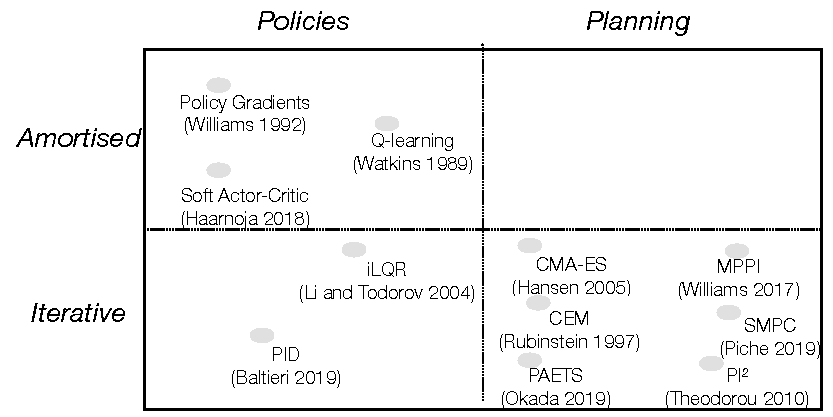
\includegraphics[width=0.8\textwidth]{chapter_4_figures/quadrant_prelim_2.pdf}
    \end{center}
    %\vspace{-0.3cm}
    \caption{Overview of classic RL and control algorithms in our scheme. Standard model-free RL corresponds to amortised policies, planning algorithms are iterative planning, and control theory infers iterative policies. The amortised plans quadrant is empty, perhaps suggesting room for novel algorithms. The position of the algorithms within the quadrant is not meaningful.}
    \label{fig:quad}
\end{figure}


\subsection{Control as Hybrid Inference}

\subsubsection{Introduction}
Building on the observation that iterative and amortised inference can be \emph{combined} to construct an iterative-amortised inference scheme which combines the advantages and ameliorates the respective disadvantages of both iterative and amortised inference -- enabling rapid and flexible inference with a high asymptotic performance, and an adaptive scheme which can leverage additional computing power only where it is most needed. In this section, we apply iterative-amortised combination to reinforcement learning which can be seen as combining model-based and model-free RL, using the identification previously developed.

Specifically, variants of model-based planning algorithms can be derived as variational inference algorithms using mirror descent to optimize the variational free energy in an iterative fashion \citep{okada_variational_2019}.
%\begin{equation}
%\begin{aligned}
%  \label{eq:vimpc}
%  q^{(i+1)}(ah; \theta) \leftarrow \frac{ q^{(i)}(ah; \theta) \cdot %\mathcal{W}(ah)\cdot q^{(i)}(ah; \theta)}{\mathbb{E}_{q^{(i)}(ah; %\theta)}\Big[\mathcal{W}(ah) \cdot q^{(i)}(ah; \theta)\Big]} 
%\end{aligned}
%\end{equation}
Additionally, as discussed previously, model-free reinforcement learning methods such as Q-learning, policy gradients, and actor-critic can be cast as optimizing another variational free energy bound, but rather this time in an amortised fashion. Given this, there are multiple potential ways to combine model-based and model-free reinforcement learning approaches. Perhaps one of the simplest approaches, which we apply in this study, is to use the model-free policy as an initialization of the model-based planner. Model-based planning algorithms such as CEM or MPPI, require an initial action distribution $p_1(a_{1:T}) = \prod_{t=0}^T p_1(a_t)$ to begin with, which they they proceed to optimize. Usually this initial action distribution is set to some simple known distribution such as a zero-centred normal distribution $p_1(a_t) = \mathcal{N}(a; 0, \sigma_a)$ with a variance parameter $\sigma_a$ which becomes a hyperparameter of the planning algorithm.

Instead, we propose to initialize the planner with the results of the amortised model-free policy network $p_1(a_t) = q_\phi(x_t)$. To do this for a potential action trajectory requires knowledge of future states to feed into the model-free policy network. However, conveniently, the model-based planner also has access to a transition model which is used to generate these simulated state trajectories, given the actions output by the policy network. 

\subsubsection{Model and Hyperparameter Details}

To make our model concrete, we need to instantiate many distributions such as the transition models $p_\theta(x_{t+1} | x_t, a_t)$, the parameterised policy $q_\phi(a_{t:T} | x_{t:T})$ and the variational iterative planning algorithm which instantiates $q(a_{t:T} | x_t; \psi)$.

The transition model was instantiated as an ensemble of three layer multi-layer perceptron networks with a hidden size dimension of size 250, which was trained to output a Gaussian distribution (mean and variance) over the \emph{change in environment state}. That is, rather than explicitly model $p(x_{t+1} |x_t, a_t)$, we instead modelled $p(x_{t+1} - x_t | x_t, (x_t - x_{t-1}), a_t)$, which we could then use to reconstruct the next predicted environmental state as $\hat{s}_{t+1} = x_t + (x_{t+1} - x_t)$. Training the transition model to predict state differences instead of the states directly is a common trick used in model-based reinforcement learning which has been found to significantly improve modelling performance by incorporating explicit information about the derivatives of the states, which is hard to derive solely from the states themselves. To obtain a measure of uncertainty over the transition model parameters $\theta$, which can be utilized to drive information-gain maximizing exploration, we maintained an ensemble of 5 transition models which were each trained on independently sampled batches of transition data. Each ensemble possessed independent randomly and uniformly initialized weights.

For the amortised action policy, we utilized the soft-actor-critic architecture (SAC) \citep{haarnoja2018soft}, with a policy-network which consisted of a three-layer MLP model with a hidden dimension of 256. We did not use an adaptive $\alpha$ parameter for the SAC agent but set it to 0.2 throughout.

For the iterative planner, we used the standard and powerful CEM algorithm \citep{de2005tutorial}, with a time-horizon of 7, a number of iterations of 10, and a trajectory sample size of 500. For each generated trajectory, to encourage more exploration, we added additional action noise sampled independently from $\sim \mathcal{N}(0, 0.3)$.

We maintained a memory buffer of all environmental interactions seen by the agent, and used various samples to train the transition model and amortised policy network. We trained the model over 10 epochs which iterated over the full memory buffer, with a batch size of 50. The full control as hybrid inference algorithm is defined as follows,
\newline 

\begin{algorithm}[H]
  \label{algo:chi}
  \SetAlgoLined
     \DontPrintSemicolon
     \textbf{Input:} Planning horizon $H$ | Optimisation iterations $I$ | Number of samples $K$ | Current state $s_t$ |  Transition distribution $p_{\lambda}(s_{t+1}|s_t, a_t)$ | Amortisation function $f_{\phi}(\cdot)$
     \BlankLine
     \textbf{Amortised Inference}: \\
    $p_{\phi}(\tau) = \delta(s_t) \prod_{t'=t}^T p_{\lambda}(s_{t'+1}|s_{t'}, a_{t'}) q_{\phi}(a_{t'}|s_{t'}; \theta)$ \\
     Extract $\theta^{(1)} = \{\mu_{t:T}, \sigma_{t:T}^2 \}$ from $p_{\phi}(\tau) $ \\
     Initialise $q(a; \theta)$ with parameters $\theta^{(1)}$
     \BlankLine
     \textbf{Iterative Inference}: \\
     \For{$\mathrm{optimisation \ iteration} \ i = 1...I$}{
        Sample $K$ action sequences $\{(a)_k \sim q(a; \theta)\}^K_{k=1}$ \\
        Initialise particle weights $\mathbf{W}^{(i)} := \{w_{k}^{(i)}\}^{K}_{k=1}$ \\
        \For{$\mathrm{action \ sequence} \ k = 1...K$}{
         $ w_k^{(i+1)} \leftarrow \frac{\mathcal{W}\big((a)_k\big) \cdot q^{(i)}\big((a)_k; \theta \big)}{\sum_{j = 1}^K \Big[\mathcal{W}\big((a)_j\big)\ \cdot q^{(i)}\big((a)_j; \theta \big)\Big]}$ \\
        $\theta^{(i+1)} \leftarrow \text{refit}\big(\mathbf{W}^{(i+1}\big)$
     }
  }
  \BlankLine
  Extract $\mu_{t:T}$ from $q(a; \theta)$ \\
  \textbf{return} $\mu_t$
  \caption{Inferring actions via CHI}
\end{algorithm}


\subsubsection{Related Work}

There has been a small amount of prior work aiming at combining model-free and model-based 
\citep{li2020robot,che2018combining}. For instance, a strand of research has focused on using a learned transition model to generate additional simulated data which can then be used to train a model-free policy `offline'. This approach was pioneered with the Dyna architecture \citep{sutton1991dyna}, but has also been extended and applied in more modern deep reinforcement learning settings \citep{gu2016continuous}. Conversely, in \citep{farshidian2014learning} and \citep{nagabandi2018neural} a model-based planner was used to initialize a model-free policy -- the opposite direction to our model. Our approach does share similarities with the approach used in AlphaGo \citep{silver2017mastering} which used learned amortized policy networks to generate proposals for the monte-carlo-tree-search (MCTS) used to select moves in that approach. However, their approach was justified on heuristic grounds and they did not consider how their approach corresponds to a mathematically principled combination of iterative and amortised variational inference. Indeed, it is not yet clear if the MCTS algorithm can be cast as performing some kind of variational inference or not.

While we are the first to consider the combination of amortised and iterative inference in reinforcement learning, and to make the connection to model-based and model-free methods, there is a line of work combining the two approaches to inference in the context of unsupervised generative modelling, typically using variational autoencoders. \citep{kim_emi:_2018}, employ amortised inference in a VAE to initialize the set of variational parameters which are then optimized directly against the ELBO. A similar approach was taken by Marino \citep{marino2018iterative}, who showed that by repeatedly encoding the gradients and optimizing the variational parameters against the ELBO, which was found empirically to improve performance and help narrow the amortisation gap.

\subsubsection{Results}

We tested our hybrid agent first on a didactic toy continuous control task. The goal of this task was to simply explore how the iterative and amortised control schemes interact. The environment was a simple 2-D planar environment, where the agent began in the bottom-left corner, and where the goal was to arrive in the top-right corner. The reward signal was a smooth gradient field leading to the top-right which was implemented as $r(x,y) = 1 - (|| (x,y) - (g_x, g_y) ||^2)$ where $g_x$ and $g_y$ represent the x and y coordinates of the goal state. In the centre of the environment there was an impassable wall except for a small opening through which the agent could pass. The agent could control its x and y velocity -- $a = (\dot{x}, \dot{y})$ with a maximum velocity of 0.05 and a minimum velocity of -0.05.

\begin{figure*}[t!]
  \centering
  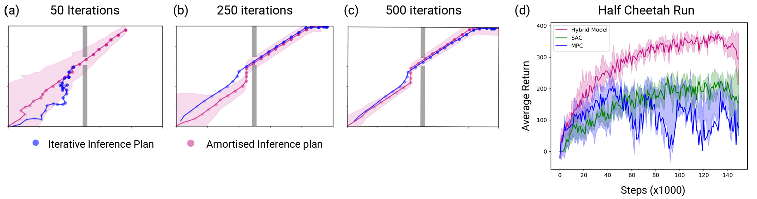
\includegraphics[width=\textwidth]{chapter_4_figures/CHI_figure_one_edit.pdf}
  \caption{\textbf{(a - c)}: Amortised predictions of $q_{\phi}(a|s; \theta)$ are shown in red, where $\bullet$ denote the expected states, shaded areas denote the predicted actions variance at each step, and the expected trajectory recovered by iterative inference is shown in blue.
  At the onset of learning (\textbf{a}), the amortised predictions are highly uncertain, and thus have little influence on the final approximate posterior. As the amortised model $f_{\phi}(\cdot)$ learns (\textbf{b}), the certainty of the amortised predictions increase, such that the final posterior remains closer to the initial amortised guess. At convergence, (\textbf{c}), the iterative phase of inference has negligible influence on the final distribution, suggesting convergence to a model-free algorithm. \textbf{(d)} Here, we compare our algorithm to its constituent components -- the soft-actor critic (SAC) and an MPC algorithm based on the cross-entropy method (CEM). These results demonstrate that the hybrid model significantly outperforms both of these methods.}
\label{hybrid_performance_figure}
\end{figure*}

The graph shows the evolution of the agent's iterative and amortised policies as it learns to complete the task. As can be seen, the iterative policy starts out highly uncertain, with a high variance. As the amortised policy is slowly learnt, the variance of the iterative policy shrinks, and the resulting policy closely matches the amortised policies. This immediately suggests an adaptive method of saving computation -- when the variance of the iterative policy is small, or the iterative policy is very close to the amortised policy, rely solely on the computationally cheap amortised policy only. Conversely, when the amortised policy or the iterative policy is highly uncertain (as at the beginning of training), then the computationally expensive model-predictive-control of the iterative policy should be utilized. In this way, the agent can attain the impressive sample efficiency and rapid performance of model-based planning at the beginning of training, when the amortised policy is poor, but then once the amortised policy becomes good, the agent can simply rely on that and thus achieve the high asymptotic performance and relative computational cheapness of model-free RL.

We also compared the hybrid agent on a challenging continuous control task -- HalfCheetah Run $\mathbb{S}^{17}, \mathbb{A}^6$. This environment requires the agent to take control of a bipedal simulated cheetah in a planar environment with semi-realistic physics. The agent's goal is to move the cheetah's limbs in such a way as to maximize the overall velocity of the cheetah, while simultaneously minimizing the total action applied. The reward function for the task was $r = v - 0.1a^2$ where $v$ denotes the overall velocity of the cheetah. The hybrid agent was evaluated against strong model-free (SAC) and model-based (CEM) baselines. As can be seen from Figure \ref{hybrid_performance_figure} the hybrid agent significantly outperforms both baselines and simultaneously achieves the sample efficiency of model-based methods with superior performance to the model-free SAC agent.

\subsubsection{Interim Discussion}

Empirically, we find that the hybrid agent performs well, and that the interaction of the iterative and amortised inference components allow for a natural adaptive scheme to switch between and apportion computation in a way that maximizes the computational resources available to the agent. Moreover, the use of an amortised policy to initialize the iterative planner cuts significantly down on the computational expense of the planner and tends to stabilize performance. Additionally, the use of the iterative planner at the start means that the agent rapidly discovers highly rewarding trajectories which are then used to train the SAC agent, and thus provides a powerful source of implicit exploration for the model-free SAC agent. Interestingly, however, this highly rewarding data generated by the iterative planner comes with a cost -- it is heavily biased towards positive trajectories, and thus the SAC agent, as it is not exposed directly to negative trajectories in the real world, simply does not learn them and thus learns a highly optimistic value function, which performs poorly when interacting with the real environment. We call this the \emph{data-bias} issue and left unchecked it inhibited the performance and learning of the algorithm.

To ameliorate the data-bias issue, we instead train the SAC agent from the simulated rollouts of the iterative planner. These rollouts, especially in the early stages of iteration, contain many examples of (predicted) negative trajectories, which thus helps render the dataset fed to the model-free SAC agent less positively biased. These rollouts do have their own difficulties -- namely that they are fundamentally from a simulation and thus may be a poor representation of the actual dynamics of the world (especially when the transition model is poor). Secondly, the rollouts are still biased to some degree by the operation of the iterative planner even in the early stages of iteration. Additionally, this becomes more acute as the model-free policy becomes better, as it learns to avoid negative contingencies and its action predictions are then used to initialize the planner, thus creating a compounding positive bias to the data that is fed into the SAC agent. Nevertheless, we find empirically that this solution suffices to train a high performance model-free policy network.

On a more theoretical level, it is important to note that we chose a relatively straightforward scheme of combination -- using the amortised policy to simply initialize the model-based planner. A more involved, but slightly more principled method may be to set the action prior of the iterative planner (which is currently assumed uniform, as is standard in the control as inference framework) to the amortised policy $p(a | s) = q_\phi(a | s)$. Using this method, instead of a direct initialization, the amortised policy would serve as a regularizer on the iterative model-based planner, ensuring that the resulting iterative policy is penalized for its divergence from the model-free amortised policy. Such regularisation methods have been found to be beneficial for the stability of learning in a number of reinforcement learning algorithms and especially in policy gradient methods, where methods such as PPO \citep{schulman2017proximal} reach state of the art performance.

\section{Conclusion}

In this chapter, we have investigated the application of methods derived from the free energy principle -- specifically \emph{active inference} -- to the general problem of optimal action selection and control. We have focused especially on a core limitation of current active inference methods: their scalability. We have demonstrated how many of the key distributions which arise out of the free energy objective can be parametrized using deep neural networks, to derive schemes which can look very similar to contemporary deep reinforcement methods -- both model-free and model-based methods. We show that these methods -- which we call \emph{deep} active inference approaches -- can perform comparably and often better to their deep reinforcement learning counterparts. 

Specifically, in the first study presented in this chapter, we showcase how active inference can be interpreted through the lens of model-free reinforcement learning. In this case, we use a learnt action policy $q(a | s)$ and parametrize the action prior using an amortized expected-free energy value network, to approximate the required path integral over the expected free energy. The resulting algorithm looks very similar to actor-critic methods in model-free reinforcement learning, but using the expected free energy instead of the reward. Additionally, we find that this approach also utilizes additional entropy regularisation terms which can be shown to substantially improve the stability and the performance of the resulting algorithm -- thus demonstrating how insights and the mathematical formalism of active inference can also lead to improvements in reinforcement learning algorithms.

In the second study, we instead approximate the path integral of the expected free energy, with monte-carlo sampling of trajectories and ultimately use a model-predictive control planning algorithm to compute optimal trajectories instead of an amortised policy network. This simple change is sufficient to move us into the realm of model-based reinforcement learning. Here, we show that active inference can again attain the performance of comparable model-based deep reinforcement learning algorithms, and can be applied to solve challenging continuous control tasks. Additionally, here the superior exploratory capabilities of the expected-free energy functional come into play, and we see that they allow the construction of powerfully exploratory \emph{goal-directed}, \emph{information-seeking} behaviours, which can solve very challenging sparse reward tasks, such as the mountain car, with ease. This demonstrates another way in which insights from active inference can aid the development of deep reinforcement learning algorithms.

We then turn to a more abstract consideration of the difference between model-based and model-free reinforcement learning in terms of inference -- an insight which is heavily enabled by the active inference formulation of action selection as fundamentally an inference problem. We demonstrate that we can see the distinction between model-free and model-based as simply that of iterative vs amortized inference, where iterative variational inference directly optimizes the parameters of the variational distribution, while amortized inference instead optimizes the parameters of a mapping function which maps observations directly to variational parameters. We then show how there is a separate dichotomy between whether policies or plans are inferred, and that this provides us with a simple two dimensional quadrant scheme upon which to place all major reinforcement learning algorithms. It also demonstrates that there are several areas which are underexplored in the literature -- especially the direct computation of amortized plans.

Finally, we use this insight into the nature of model-based and model-free reinforcement learning in terms of iterative and amortized inference to ask how these two approaches can be \emph{combined}. We show that this can yield powerful algorithms which can combine both the sample-efficiency and rapid learning of model-based planning with the asymptotic performance and computational cheapness of model-free reinforcement learning. Importantly, investigations into this field of combined or hybrid reinforcement learning algorithms are only just beginning, and there are many design choices left to be extensively investigated in future work.

Overall, crucially, we have shown that the free energy principle and active inference can be successfully applied and scaled up to handle large and challenging control tasks and to create algorithms which perform comparably with state of the art methods in deep reinforcement learning.

In the next chapter, we extend the intuitions provided here about the importance of combining exploration and exploitation and turn to a more abstract and mathematical analysis of what kind of mathematical procedure gives rise to the combination of exploratory and epistemic action that characterise such objective functionals as the Expected Free Energy and the Free Energy of the Expected Future. 